\chapter{GROUPING RNA 3D STRUCTURE FILES IN MMCIF FORMAT INTO EQUIVALENCE SETS}

\section{Introduction}

This chapter reports changes implemented to improve modules of the data pipeline
that calculates Equivalence Classes of RNA entities of RNA 3D structures for the
Nucleic Acids Database (NDB) and for RNA.BGSU.EDU. The 3D structures are
provided by the Protein DataBank (PDB).

The PDB serves as the archival resource for the accumulated scientific
investigations of the 3D structures of macromolecular entities of biological
significance carried out by scientists all over the world. The earliest entries
date back to the late 1960s and early 1970s and new entries are accumulating at
an ever-increasing rate. The earliest RNA entries were structures of
dinucleotides and the latest entries include entire ribosome and splicesome
structures bound to a variety of tRNA and mRNA substrates and translation
factors. But structures containing smaller RNA molecules bound to enzymes that
modify them or use them as guide RNAs  to recognize other substrates continue to
accumulate. For example structures of CRISPR complexes recently started to
appear \cite{Wang2015, Nunez2015}. Thus there is a huge variation in the size of
the RNA entities and of the scientific purposes for which the investigations
were conducted.

\section{Previous work}

We have previously implemented a method to group RNA molecules into equivalence
sets. The method is described in a book chapter entitled ``Nonredundant 3D
Structure Datasets for RNA Knowledge Extraction and Benchmarking''
\cite{Leontis2012b}. The current work is an extension of these methods so, we
begin by briefly describing the previous methodology which was developed when 3D
structures were still distributed in PDB files, so that large structures like
70S ribosomes had to be split over two or more PDB files. At that time it was
convenient to simply select the largest RNA chain in each file to represent the
RNA in the file for grouping. In cases where the file also had one or more
smaller RNA chains the smaller ones were simply ignored and no groups built for
them. For example, structures of large ribosomal subunits contain both the 23S
and the much smaller 5S rRNAs in the same file, but the 5S was simply ignored
and not extracted and clustered at all. Each extracted chain was compared on the
basis of sequence alignment, species and geometric discrepancy to all other
chains. The previous method did not compute all possible sequence alignments or
discrepancies, due to limitations imposed by runtime. The alignments and
geometric discrepancies of chains in the same group were not stored for future
studies.

\section{Motivation for current work}

We have two main motivations for updating our RNA chain grouping method. The
first is to take advantage of technical changes data and the second is to
enhance the scientific utility of our resources by providing a more complete set
of data that includes all chains found in RNA structures.

Recently, the PDB resource management team has migrated from using outdated,
80-column wide ``PDB''' formatted structure files to the new modern-style
macromolecular Chemical Information File format (mmCIF), which makes it possible
to store structural information for macromolecular complexes of any size in just
one computer file. By contrast, the out-dated PDB format was limited to no more
than 99,999 numbered atom data records per file. This change has made possible
the storage for example, of entire ribosomes in a single file, including both
the large and small subunits, tRNA, mRNA fragments, 5S and 5.8S rRNA (for
eukaryotes). In some files such as 4V4Q \cite{Schuwirth2005} more than one
entire ribosome is present. Because our old method only considered the largest
chain in each file the old method would ignore all chains except a single LSU
rRNA when processing mmCIF files. This would lead to ignoring many important
groups of RNA structures. The new method extracts and classifies all RNA chains
from all mmCIF files.

There are a number of scientific use cases for which our RNA structure classes
and derived data will be  3D structures in the PDB/NDB and these are worth
enumerating and discussing.

\begin{enumerate}
  \item Determining the breadth and depth of solved structures, i.e. the number of
    distinct types of RNA and the number of instances of each type.

  \item Statistical studies of recurrent elements of RNA structure, RNA-RNA and
    RNA-protein interactions

  \item Comparative studies of similar or homologous RNA structures and
    RNA-protein complexes

  \item Functional studies of RNA structural flexibility, variation and
    conformational change in response to environmental perturbations

  \item Comparative assessment of RNA structure modeling quality and reliability

  \item Compilation of modular RNA parts for synthetic biology and RNA
    nanotechnology

  \item Analysis of RNA sequence variation to improve RNA structure prediction
    and understanding of RNA evolution
\end{enumerate}

Thus, the change to mmCIF format required a complete rethinking of the
procedures for extracting, naming, and clustering RNA entities and has enabled
significant improvements in the results. This chapter describes those changes
and the choices made to maximize the value of the data for diverse scientific
users.

\section{Types of molecules and requirements}

In this section we will highlight specific groups of RNA molecules that pose
special challenges for clustering to motivate the following sections, where the
methods developed are explained and their success in clustering appropriately,
these special cases is assessed.

\subsection{Ribosomal RNA subunits}

Among the largest entities are ribosomal RNAs (rRNA), which include the rRNA of
the large (LSU) and small (SSU) ribosomal subunits, the 5S rRNA, and the 5.8S
rRNA in eukaryotes. LSU and SSU rRNA from a number of species representing all three
major phylogenetic domains and mitochondria are presently available in PDB/NDB.

The rRNAs should be divided into separate Equivalence Classes (EC) as follows:
First, each of the SSU rRNAs (mitochondrial 12S, bacterial 16S and eukaryal 18S
rRNAs) should be placed into their own EC by organism. Further, each of the 23S
rRNAs from archaeal or eubacterial ribosomes should be placed in distinct EC.
The 5S rRNAs, which are found in the LSU of all ribosomes except some
mitochondrial ones, should also be in separate groups. While bacterial 5S rRNA
does interact directly with 23S rRNA in the LSU, it does so through
non-Watson-Crick pairing and backbone interactions involving its ``loop E''
internal loop (IL) motif and a similar structured IL in helix 38 of 23S rRNA.
The loop E, as well as the rest of molecule, of 5S rRNA has been shown to assume
the same 2D and 3D conformation in the absence of 23S rRNA and so is not
dependent on 23S to form its native state. The same holds for eukaryal 5S rRNAs.
Therefore each 5S rRNA is placed in its own EC independently of the 23S rRNA.

By contrast 5.8S rRNA found in eukaryal LSU, constitutes an integral part of the
large rRNAs (26S or 28S, depending on the species), as the 5.8S molecules are
homologous to the 5'-ends of bacterial 23S rRNAs. As such, they form extensive
Watson-Crick interactions with the larger 26S or 28S rRNA of the LSU and so,
according to the criteria defined above, belong together with the large rRNA in
the same RNA entity for the purposes of grouping.

In addition, the structure of the ribosome has studied sever since it was
discovered in the 1950's \cite{McQuillen1959, BEER1960, ABDUL-NOUR1960,
OHTAKA1963, SANTER1963}. Early structures \cite{Mueller2000} often were resolved
at very low resolution use electron-microscopy. These structures, while
informative, are not as useful for detailed structural analysis as more recent
high resolution structures. While we intend to group all structures, it is very
useful to create separate structures into groups with similar resolution. In the
past, we have found using resolution cutoffs of 1.5{\AA}, 2.0{\AA}, 2.5{\AA},
3.0{\AA}, 3.5{\AA}, 4.0{\AA}, 20.0{\AA}, for grouping is useful A catchall group
of resolution includes all structures. Here we continue this practice.

From these examples we can see that the members of groups of structurally
similar RNA entities should comprise one or more chains which interact
extensively through Watson-Crick base pairing. These should be considered a
single entity and then grouped with other such entities. Furthermore, each group
should only contain RNA entities from the same species. Thus 16S rRNA from \EC{}
and \TT{} are assigned to distinct equivalence classes (EC). In the case of
large molecules, this can be determined through sequence alignments alone. In
addition, all members of a group should meet a resolution criterion.

\subsection{tRNA and mRNA complexes}

Structures of tRNA molecules are often found in the context of their binding to
ribosome structures. In ribosomes, they are usually also bound mRNA fragments.
These mRNA fragments span at least the A and P sites of the rRNA and have more
than one tRNA's bound. The smallest mRNA fragments (6 bases) are extensively
bound to the tRNA as all bases are paired with the tRNA. Despite the extensive
pairing we choose not to place the tRNA's and mRNA into a single entity for
grouping as these interactions are transient, unlike the case for the 5.8S. In
this case we believe the most scientifically meaningful unit is the tRNA. The
small mRNA fragment is not interesting alone from a structural viewpoint. It is
small and lacks internal structure. Thus, while we do want to place two chains
which extensively pair into a single unit (e.g. 28S+5.8S rRNAs) we do not
consider it meaningful to allow small unstructured chains connect two larger
structured chains. For the purposes of grouping all chains we allow the small
unstructured chain to ``accompany''' each of the larger chains individually, but
not to connect the two structured chains. However, they are also found bound to
tRNA-modifying enzymes, translation factors or by themselves into a single
larger entity.

The tRNA case also provides another case to consider. It is well known that some
initiator tRNA's from different species have the same sequence. This implies
that sequence alignments alone cannot separate molecules from different
organisms into separate EC's. However, most authors provide ``source organism''
annotations. Investigations into such annotations have shown that while many are
precise, others are annotated with ``synthetic compound''' or are not provided.
These chains often have sequences identical to other annotated chains. In other
cases, the synthetic chain aligns very well to a correctly annotated chain. Thus
we can treat molecules annotated ``synthetic''' or lacking any annotation as
being similar to any other annotated species.

The fact that some molecules from different organisms will have identical
sequences, and the potential issues with author annotations shows us that while
we should use alignments and organism assignments to place RNA entities in the
same group, we must provide another criterion. We must enforce that each EC
contain a single species, ignoring the annotations ``synthetic''. This will
enforce our requirement that groups contain only members from the same species.

\subsection{Small model compounds}

A great deal of detailed structural information has been provided by studies of
small model constructs. These entities are often composed of two molecular
strands which bind to form a small helix sometimes having an internal loop. For
example, studies of the isolated sarcin-ricin motif \cite{Olieric2009} have
provided detailed information on its structure. In these structures the relevant
unit to is the duplex not the individual strands. Like the LSU and 5.8S each
strands interact extensively through Watson-Crick base pairs with it's partner.
However, these strands generally lack internal structure. There are also model
constructs containing more than 2 strands for example, such as the nano square
that are comprises of 8 chains \cite{Dibrov2011a}.

From these examples we can see that we should be able to join any number of
unstructured chains tat form extensive pairing interactions together to form a
single unit for grouping. This is different from the case of multiple tRNA's on
a small mRNA fragment where the two tRNA's would not form a single unit. Here we
want to join the chains, even though they do not interaction directly withe ach
other, to form a single unit.

Many of these small model constructs differ from one another only by a single
nucleotide change. These changes are intentional and meaningful and so we
require that small constructs have identical sequences to belong to the same
group. In this way, small constructs differing even by one nucleotide are
assigned to separate groups.

\subsection{Small Protein and RNA complexes}

Several proteins have been solved bound to  small RNA's. These RNA's are often
single-stranded and in some cases homopolymers, e.g. poly-A. Such low-complexity
chains may agree in sequence and species assignments but they differ in assigned
geometry due to binding by different proteins. These chains should be placed in
separte groups even though the sequences and species are indtical, because of
the large structural changes. Thus our groupings should be sensitive to the
overall geometry of the members.

\section{Criteria for equivalence classes and their members}

These examples, show first of all, that many CIF files contain more than one
chain. Secondly, the example of Eukaryotic LSU rRNA shows that the members of
some EC comprise more than one chain in contrast to our previous EC. A
prerequisite of grouping is to define the RNA-containing entities to be
extracted from structure files as precisely as possible and in a manner that is
biologically relevant for the purposes of most users of the NDB resource. Guided
by the importance of prioritizing biological relevance, we settled on the
following definition of the relevant RNA-containing entities for clustering into
EC: The entities to be identified and extracted from PDB/NDB structure files
should be ``groups of one or more RNA chains that form identifiable, integrated
structural and functional units.''' Internally we refer to these entities as
``RNA integrated functional elements''' or RNA ``IFE's.''' We will use the term
``IFE''' as a short-hand for this definition.  Most RNA IFE's consist of a single
chain, but some do not in fact there is no predefined limit to the number of
chains. The simplest examples comprise two Watson-Crick paired chains
forming a duplex structure: strictly speaking, they comprise two molecules, but
effectively the form a single entity, i.e. RNA IFE.

From these examples we can see there are three requirements for each EC.
\begin{description}
  \item[Biological Source] Two IFE's included in the same Equivalence Class
    should come from the same biological source. The intention of this criterion
    is to separate homologous RNA molecules, for example, SSU rRNA's from
    different organisms, into distinct Equivalence Classes.

  \item[Sequence Similarity] Two IFE's included in the same EC should have very
    similar, though not necessarily identical sequences. This criterion may seem
    redundant with the first criterion. The intention is to include sequence
    variants (for example 16S rRNAs coded by different genes of the same
    micro-organism that differ in a small number of positions) but to separate
    molecules with similar sequences from evolutionarily related organisms that
    belong to distinct species. We note that not all RNA chains in PDB are
    labeled with a biological source, which complicates clustering by this
    criterion.

  \item[Geometric Similarity] Two IFE's included in the same Equivalence Class
    should have the similar conformations and geometries. The intention of this
    criterion is to separate instances in which there is a significant
    conformational change, even when the RNA sequence(s) and biological sources
    are the same. For example, poly-A bound to poly-A binding protein (PAB) (PDB
    1CVJ \cite{Deo1999}) has a different conformation from poly-A forming a
    parallel strand duplex (PDB 4JRD \cite{Safaee2013}). These IFE's are
    structurally dissimilar and should not be in the same equivalence set, even
    though the sequences may be identical.

  \item Resolution: Two IFE's included in the same EC should be in the same
    resolution range.
\end{description}

The reader should note that we decided to group structures together even though
their sizes differ when these criteria are met:

\begin{enumerate}
  \item When the same molecule is used in the experiment, i.e. as the
    experimental sequence, as reported in the mmCIF data as
    ``poly\_seq\_scheme'', but the observed molecules differ in size. In some
    cases only part of the molecule is resolved in a 3D structure. We have
    decided that whenever the same RNA is used in different experiments, the
    resulting IFE's should be clustered in the EC even though the observed
    sequences may differ in size.

  \item In addition, the observed part superposes well with the corresponding parts of
    more completely resolved structures.

  \item When the observed structure is a small part of the overall molecule. For
    example, there are structures of a single domain of 16S rRNA or 23S rRNA
    \cite{Nissen2000}. These structures are best grouped with the corresponding
    complete 16S or 23S rRNA, as that is the context they are just a small
    portion of the larger complex.
\end{enumerate}

In addition, there are several other cases where we assign IFE's to the same EC:

\begin{enumerate}
  \item We group IFE's together EVEN WHEN their geometries differ significantly,
    if the structures are solved at such low resolution that the data are inadequate to
    quantify the structural differences.

  \item RNA entities belong together even when they are bound to different proteins
    or ligands as lng as they have very similar geometries. At present,
    it is not our intention to classify PDB structures at the level of
    RNA-protein complexes. For this study we focus on the RNA components of the
    structure. In this way tRNA's from the same organism and species bound to
    different proteins will be placed in the same EC unless the protein
    significantly distorts the structure.
\end{enumerate}

There are several important implications of these requirements. First it is
possible that the homologous RNA molecules (for example iso-accepting tRNA's)
from different species have nearly identical sequences and structures.
Nonetheless they will be placed in different groups. In addition, it is possible
that two EC will contain IFE's having similar sequence and species but differ
only in geometry.

\section{Methodology for building Equivalence Sets}

In this section we discuss the process of building EC's. The overall process
comprises these three steps:

\begin{enumerate}
  \item Identify and extract RNA chains from all mmCIF files

  \item Identify interaction chains and build RNA IFE's from individual chains.

  \item Link pairs of IFE's by sequence similarity, source species, and
    geometric similarity to form initial EC

  \item Extend EC using transitivity of similarity links

  \item Assign names and group by resolution

  \item Display data on our RNA.BGSU.EDU

  \item Share data with NDB
\end{enumerate}

Next we discuss each step in detail and how it achieves our goals.

\subsection{Building RNA IFE's from individual chains}

We have implemented an algorithm for joining RNA chains extracted from the same
mmCIF files into IFE's. As discussed in our examples, the joining logic depends
on whether the chains are ``structured''. Structured chains only get joined with
other structured chains they directly interact with, and they must make a
significant number of interactions with each other. Unstructured chains are
always joined to any chain with which they interact, but they are not allowed to
indirectly join two structured chains to one another to form an IFE.

Our algorithm operates as follows. We first mark all chains in a structure as
``structured''' or ``unstructured''. A ``structured'' chain is defined by having
at least 5 internal \emph{cis} Watson Crick/Watson Crick (cWW) basepairs.
Internal basepairs are defined as forming between nucleotides belonging to the
same chain. We then join chains based upon four rules. A representation of
these rules is shown in Figure~\ref{fig:build-ife} and pseudocode for the logic
is shown in Figure~\ref{fig:pseudo-ife-building}.

\begin{figure}
  \includegraphics[width=\linewidth]{chapter-3/figs/build-ifes}
  \caption{The rules for connecting chains into IFE's. Each chain is
    represented by a circle. Unstructured chains are in blue with the letter
    ``U'', while structured chains are orange and labeled ``S''. The left side
    indicates the input and the right shows the possible results of joining
    chains in different cases. On the left the dotted lines indicate one or more
    cWW interactions between the chains. On the right each grey oval indicate
    an IFE built of the two chains. For case 1 and 2 we always join the two
    chains into one IFE, while in case 3 joining depends upon the number of
    interactions. Case 4 shows that for two structured chains selected by an
    unstructured chain the two structured chains are placed in separate IFE's
    while the unstructured chain is included in both IFE's.}
  \label{fig:build-ife}
\end{figure}

The logic for joining chains into IFE's is as follows:

\begin{description}
  \item[Rule 1] Always connect two unstructured chains that form cWW basepairs
    to one another. This
    allows for joining of separate stands of duplexes.

  \item[Rule 2] Always connect unstructured chains to structured chains with
    which they form cWW basepairs with. This serves to connect unstructured
    fragments such as mRNA's to the structure tRNA's they are interacting with.

  \item[Rule 3] Connected to structured chains if the maximum ratio of internal
    to external cWW pairs is at least 0.6. This is an experimental determined
    cutoff. It may be adjusted in the future as needed. To examine if this
    cutoff is reasonable we produced the figures shown in
    Figure~\ref{fig:ext-vs-int}.

  \item[Rule 4] If two structured chains are connected indirectly by an
    unstructured chain, place the unstructured chain with both structured chains
    as an ``accompanying'' chain but do not join the two structured chains.
\end{description}

\begin{figure}
  \begin{tabbing}
    Fore\=ach p\=air of chains \\
      \>If the chains do not interact \\
      \>\>Skip \\
      \>End \\
      \>If one chain is unstructured \\
      \>\>Join chains \\
      \>Else If both are structured and internal/external > 0.6 \\
      \>\>Join chains \\
      \>End \\
    End \\
    Foreach grouped chain \\
    \>If two structured chains do not interact \\
    \>\>Split the structured chains \\
    \>End \\
    End
  \end{tabbing}
  \caption{Pseudocode for the logic of joining chains into IFEs. This is a more
  structured representative of the logic shown in the Figure~\ref{fig:build-ife}.
  }
  \label{fig:pseudo-ife-building}
\end{figure}

\begin{figure}
  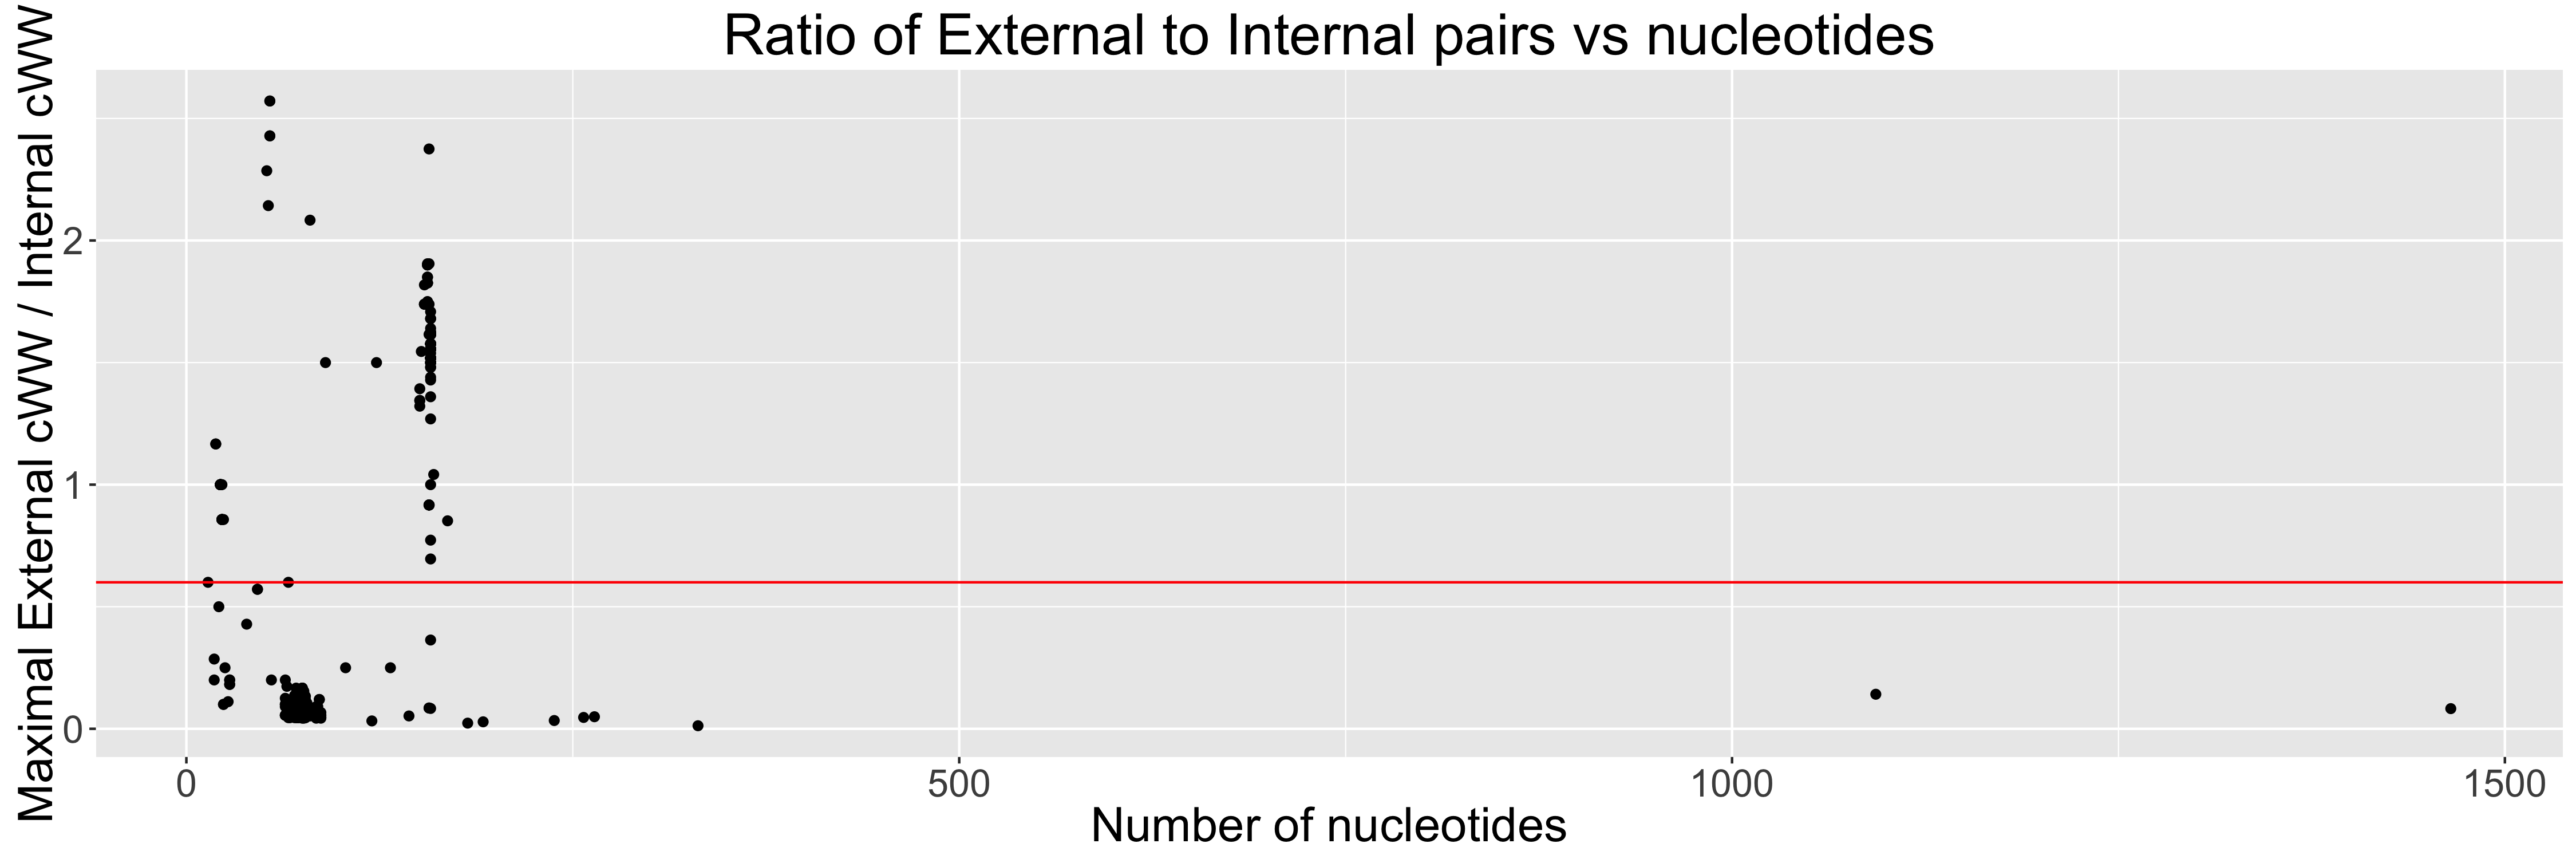
\includegraphics[width=\linewidth]{chapter-3/figs/internal-external}
  \caption{Summary of the ratio of external to internal base pairs. The leftmost
    panel shows a histogram of the maximal ratio of external to internal pairs
  for all pairs of chains which have an interaction between them. }
  \label{fig:ext-vs-int}
\end{figure}

\subsection{Connecting pairs of IFE's to from equivalence sets}

To build equivalence sets we compare all pairs of IFE's in the preliminary list
based upon their species assignments, their sequence alignments, their geometric
discrepancy. Pairs of chains which have a valid alignment, and identical
biologic source (or from a synthetic source) and have a geometric discrepancy of less than
0.4{\AA}, if computed, are joined. As mentioned above we do not compute
discrepancies for chains with very low resolution. The discrepancies computed
for one or more chains with low resolution, greater than 5{\AA}, are artificially
inflated. These artificially high values will cause IFE's that are similar end
up split into different groups incorrectly. We then build the EQ sets by placing
all chains which are transitively connected into one set. 

The steps are:
\begin{enumerate}
  \item Determine the species assignment for all chains.
  \item Compute the alignment of all pairs of alignable chains.
  \item Compute the geometric discrepancy between all chains which have a good alignment
\end{enumerate}

The first step requires looking up the assigned taxonomy for chain. Many chains
are assigned to a particular species making the lookup trivial, however some are
also assigned to a subspecies. For these cases we use the parent species of the
chain ignoring subspecies. However, not all chains are assigned to an organism,
as many are marked as ``synthetic construct''' or not assigned any organism. In
both of these cases we treat the organism as synthetic. In addition, a few
chains (3) are assigned to a genus rather than a species or sub-species, in
these cases we treat the chain as being synthetic as well. We do not treat
synthetic chains specially except when comparing to another annotation. In the
case of comparing a synthetic chain to another chain the two are always
considered to have the same species.

In order to compute the alignments between all pairs of chains correctly and in
a reasonable time frame, we align experimental sequences and not observed
sequences. Experimental sequences are the sequences used in the experiment and
may differ from what is observed in the experiment. The experimental sequence is
found in the mmCIF field labeled ``pdbx\_poly\_seq\_scheme'' and the observed
sequence is mapped to the experimental in that field as well. Often the observed
sequence will have ``gaps'' in 3D indicating where bases were not resolved. For
example 4V54  Chain DB has no coordinates for residues 879 to 897
\cite{Borovinskaya2007a}. In order to build alignments consistently we use the
experimental sequence. If we did not we would have to ensure that the resulting
alignments respected possible gaps in all chains. The alignments would  have to have
breaks where the observed chains have breaks. This is a difficult problem and it
is simpler to use the experimental sequences, where this is not a concern.

In addition, by using experimental sequences we reduce the number of required
alignments. It is very common to use the same molecule in many experiments. For
example, there are many structures of the same \EC{} rRNA bound to different
tRNA's or antibiotics. All of these structures can be represented by a few
experimental sequences. There is no need to realign sequences simply because
they came from different experiments, as the alignments made using experimental
sequences remain the same.

Before aligning two experimental sequences we check that they have similar size.
The rules for size similarity depend upon the size of the chain and are shown in
Table~\ref{tab:size-rules}. The reason for the size constraint is to avoid
unnecessary alignments while ensuring that we perform all needed alignments. For
example, attempting an alignment between a large and small rRNA subunit is
unnecessary and should be avoided. In addition, aligning a three nucleotide mRNA
fragment to an LSU may produce a match, but the match is meaningless. By imposing
size rules we also eliminate meaningless alignments. We have a hard limit 

\begin{table}
  \begin{tabular}{lr}
    \toprule
    Sequence Size & Size Rule \\
    \midrule
    $s < lt 19$          & Same Size                         \\
    $19 \leq s < 2000$ & Within 50\% and less than 2000    \\
    $2000 \leq s$        & Within 50\% and greater than 2000 \\
    \bottomrule
  \end{tabular}
  \caption{List of rules used when selecting the pairs of sequences to align. In
  the columns $s$ is the length of the shortest experimental sequence}
  \label{tab:size-rules}
\end{table}

Finally, we require that two experimental sequences either be assigned to the
same species or to ``synthetic'' before we attempt to align them. We refer to
this condition as the chains having a ``similar species''. This ensures that we
are only comparing sequences which could possibly be from the same biological
source. We have observed that some experimental sequences are assigned
``synthetic'' in one experiment but annotated a specific organism in another
experiment. Thus we allow the comparison of synthetic chains to any other chain,
so long as it has similar size. 

The last step is to compute the geometric discrepancy. Geometric discrepancy is
a measure of geometric similarity, like RMSD but it is sensitive to the base
orientation and position. It has been used extensively in our research group for
searching RNA 3D structures \cite{Sarver2008a}, building NR sets in the past
\cite{Leontis2012b}, as well as building RNA motif groups \cite{Petrov2013}. We
only compare the largest, most structured (most basepairs per nucleotides) chain
in each IFE to compute geometric discrepancy. While this is a simplification of
the situation it has proven to work well and makes the problem simpler. If we
did not do then we would have to determine which chains in the IFE's to compare.
This can be difficult in some IFE's and produces marginal benefit. For geometric
discrepancy we are only interested in chains that:

\begin{enumerate}
  \item Have a good alignment between them. As this geometric discrepancy will
    be used to build the EC, there is no need to compute it for chains that do not
    align well. These chains cannot be in the same EC so geometric
    discrepancy is not needed. This reduces the number of comparisons needed,
    reducing the number of computations to complete.

  \item Have resolution less than 4.0{\AA} or are solved using NMR. We do not
    compute geometric discrepancies for chains with resolution greater than
    4.0{\AA} because doing so provides artificially inflated discrepancy values.
    Many structures of low resolution are helices which have not been modeled
    with planar paired bases. This modeling is inaccurate and produces high
    geometric discrepancy when compared to carefully modeled helices. If the
    program use the artificially inflated values, it will split structures which
    should be joined. Thus we do not compute discrepancies for structures that
    We do however allow for comparisons using NMR because most of the structures
    are quite small. Small chains tend not to have artificially inflated geometric
    discrepancy values.

  \item Have at least 3 aligned bases. This is because geometric discrepancy is only
    defined for at least 3 bases. Thus very small structures (2 or less
    nucleotides) are not compared.
\end{enumerate}

With these rules we are able to efficiently compute all required discrepancies.
This is done as part of our pipeline when structures are imported from PDB and
the values are stored in our database. This allows for subsequent comparison of
grouping methodologies and constraints.

We then connect all pairs of IFE's which satisfy the alignment, species and
geometric discrepancy requirements. These connections are treated as a graph and
used to build EC through transitivity.

\subsection{Building equivalence classes from pairs of IFE's}

We build EC through transitivity. This means that all connected IFE's, even if
the connections are indirect, are placed into a single group. It is not required
that each IFE be connected to every other IFE to form a complete graph. An
example of such a clustering is shown in the left panel of
Figure~\ref{fig:transitivity}.

\begin{figure}[ht]
  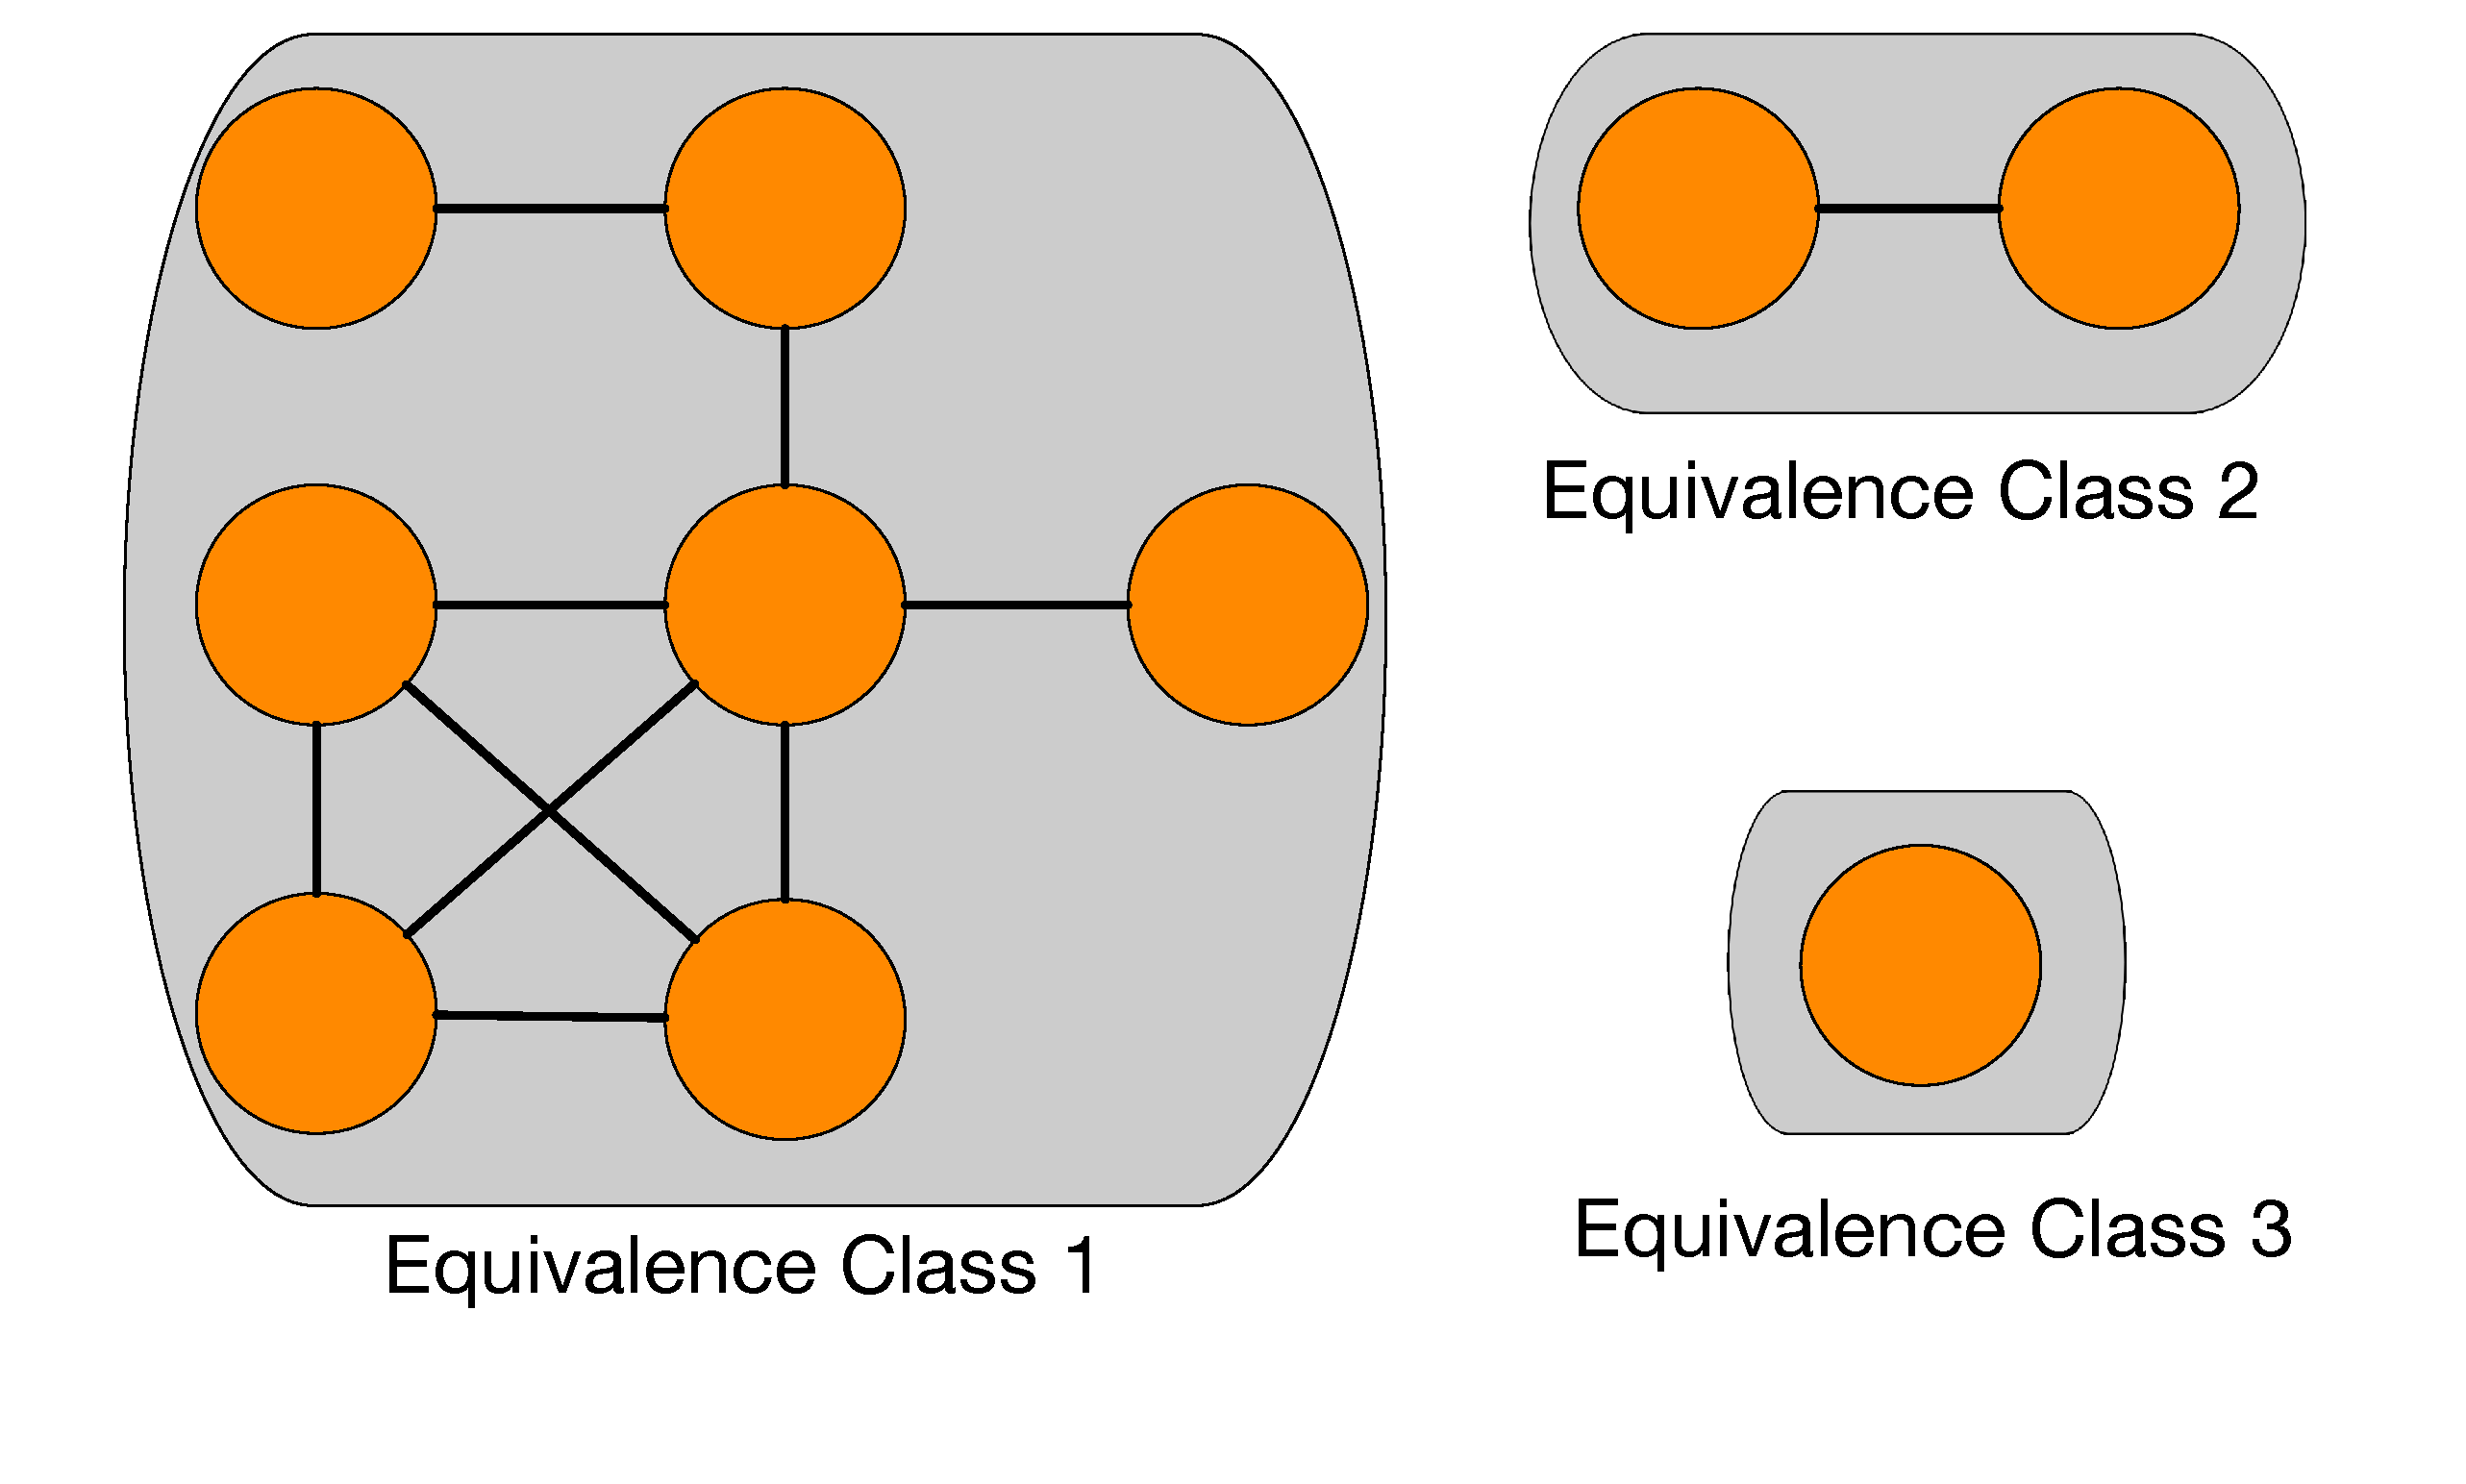
\includegraphics[width=\linewidth]{chapter-3/figs/ife-transtivity}
  \caption{Schema of Equivalence Classes built by transitivity. In this figure
    each IFE instance is represented by a circle. Lines connecting circles
    indicate pairs of IFE's having similar sequences, the same species and
    geometric discrepancy below the threshold value of 0.4. Each Equivalence
  Class is represented by the grey background around a set of circles. To in
included in a class an instance need only be connected to one other member of
the class.}
  \label{fig:transitivity}
\end{figure}

Using transitivity to include IFE's that are not maximally connected minimizes
the number of singleton groups. The remaining singletons are true outliers in
not being connected to any other IFEs. Most IFE's will be connected to at least
one other IFE, placing them in some group. Without transitive grouping,
IFE's that differ only from one other IFE in a group would be placed in their
own EC.

Initially, the groups are created using structures of all resolutions, the
``all'' resolution cutoff. Each group is then filtered at each resolution cutoff
(1.5{\AA}, 2.0{\AA}, 2.5{\AA}, 3.0{\AA}, 3.5{\AA}, 4.0{\AA}, 20.0{\AA}) to
remove IFE's above the resolution cutoff. Once the EC are partitioned by
resolution the final step is to name them.

\subsection{Naming Equivalence Classes}

In previous work, Dr. Anton Petrov created a naming scheme for EC based upon the
parentage of the equivalence class \cite{Petrov2013}. I preserve the overall
scheme, but modified it in a significant way to produce an easier to understand
system, as described next.

The naming schema is as follows:
``NR\_{resolution\_cutoff}\_{unique\_handle}.{version}''. This schema has three
components, the resolution cutoff used, a unique randomly selected handle
consisting of 5 digits and the version number for this EC. The resolution cutoff
provides information on what the resolution is used to build the EC. The unique
handle is a unique randomly generated 5 digit number that serves to make all ids
unique.

We have changed the naming scheme so that the unique handle is identical across
all resolution cutoffs of the same EC. For example, an EC built of tRNA's at the
``all'' resolution cutoff having the name: ``NR\_all\_00001.1'' will now have
the name ``NR\_4.0\_00001.1'' to designate all structures better than 4.0{\AA}
resolution. This differs from the previous method where different randomly
generated handles were assigned to each resolution cutoff of the same EC. By
making this change the random handle remains identical across resolution cutoffs
making it possible to determine from the name EC have the same IFE's.

\section{Results of Equivalence Class building}

For the purposes of this chapter we created an EC grouping using all structures
available as of July 25, 2016. This grouping was then analyzed to determine
whether the resulting groups met our objectives. I begin with a general
description of the clustering and then discuss each previously mentioned special
case in detail; finally, I examine the groupings of outliers.

\subsection{General properties of the new Equivalence Classes}

I built a EC grouping using all mmCIF files from PDB available as of July 28,
2016. The grouping used 3213 mmCIF which contained 7015 IFE's. These were
grouped by the new procedure into 2168 EC's. These groups varied in number
of IFE's from 1 (singleton groups) to 377 IFE instances. A summary of the
member count distribution is shown in in Table~\ref{tab:eq-size-dist}.

\begin{table}
  \begin{tabular}{lr}
    \toprule
    Number of instances & Number of Equivalence Classes (Percent of all classes) \\
    \midrule
    1               & 1352 (62.4\%) \\
    2-5             & 615 (28.3\%)  \\
    5-10            & 118 (5.4\%)   \\
    10-20           & 53 (2.4\%)    \\
    20-50           & 16 (0.7\%)    \\
    \textgreater 50 & 14 (0.6\%)    \\
    Total           & 2168 (100\%)  \\
    \bottomrule
  \end{tabular}
  \caption{Counts of the number of classes for a range of sizes. This table
    shows the number of classes for a range of sizes for the new grouping method
  for all 3213 structures available as of July 28, 2016}
  \label{tab:eq-size-dist}
\end{table}

The table shows a surprisingly high percentage, 62\%, of singleton groups. I
tested to determine whether the new method is consistent with the previous
method by building a grouping using the set of PDB files December 05, 2014 as
shown in Table~\ref{tab:compare-size-dist}. This date was chosen because it
corresponds to both the last grouping using our previous method as well as the
transition to mmCIF data. These two datasets contain the same experimental
results, however there are fewer mmCIF files than PDB because many of the PDB
files were merged into larger mmCIF files. This gives us an ideal data set to
compare the two methods. Table~\ref{tab:compare-size-dist} shows that the old
and new methods have similar performance, although the new one produces slightly
fewer singleton groups (1081 vs 1112). Thus 62\% of our groups are singleton
groups for the July 28, 2016 data is not surprising when compared to the
previous groupings. There is a bigger difference in the percent of singletons
however (61\% vs 78\%). This is due to the fact that the new method produced
significantly more EC (1765 vs 1409) because more IFE's are extracted by the new
method.

\begin{table}
  \begin{tabulary}{\linewidth}{LRR}
    \toprule
    Number of instances &
    Number of Equivalence Classes in 2.0 &
    Number of Equivalence Classes in 1.89 \\
    \midrule
    1               & 1081 (61.0\%)  & 1112 (78\%) \\
    2-5             & 527 (30.0\%)   & 234 (16\%)\\
    5-10            & 88 (5.0\%)     & 31 (2\%)  \\
    10-20           & 38 (2.0\%)     & 19 (1\%)  \\
    20-50           & 20 (1.0\%)     & 8 (0.5\%) \\
    \textgreater 50 & 11 (0.6\%)     & 5 (0.3\%) \\
    Total           & 1765 (100\%)   & 1409 (100\%) \\
    \bottomrule
  \end{tabulary}
  \caption{Comparison clustering IFE's into EC using the new method and previous
  method on the same data set. This table compares the performance of the
  previous and new method on the same data set of structures. The data are taken
  from \URL{http://rna.bgsu.edu/rna3dhub/nrlist/download/2.0/all/csv}, which
  contains 2680 structures, and
  \URL{http://rna.bgsu.edu/rna3dhub/nrlist/download/1.89/all/csv} (contains
  3145 structures) and represents all the structures available as of
  December 5, 2014. The transition from 1.89 to 2.0 corresponds to the
  move from PDB to mmCIF formats, which decreased the total number of
  files, because many previously separate files were merged}
  \label{tab:compare-size-dist}
\end{table}

I next moved to examine results of EC's of particular interest. I begin with
the ribosomes, then tRNA's, and then other protein/RNA complexes.

\subsection{Ribosomal subunits}

As an example to evaluate the grouping in to EC of rRNA, I examined the EC
containing the \TT{} small ribosomal subunit (SSU). We constructed heatmaps of
both the sequence similarity and the geometric discrepancy between all 16S IFE's
as shown in Figure~\ref{fig:tt-ssu-align} and Figure~\ref{fig:tt-ssu-disc}. The
alignment heatmap indicates high sequence similarity among all IFE's. The
geometric discrepancy heatmap shows that there may be two main structurally
distinct groups in the \TT{} 16S EC. Currently we are exploring these groups to
determine whether if they correlate to functionally distinct states.

\begin{figure}[h]
  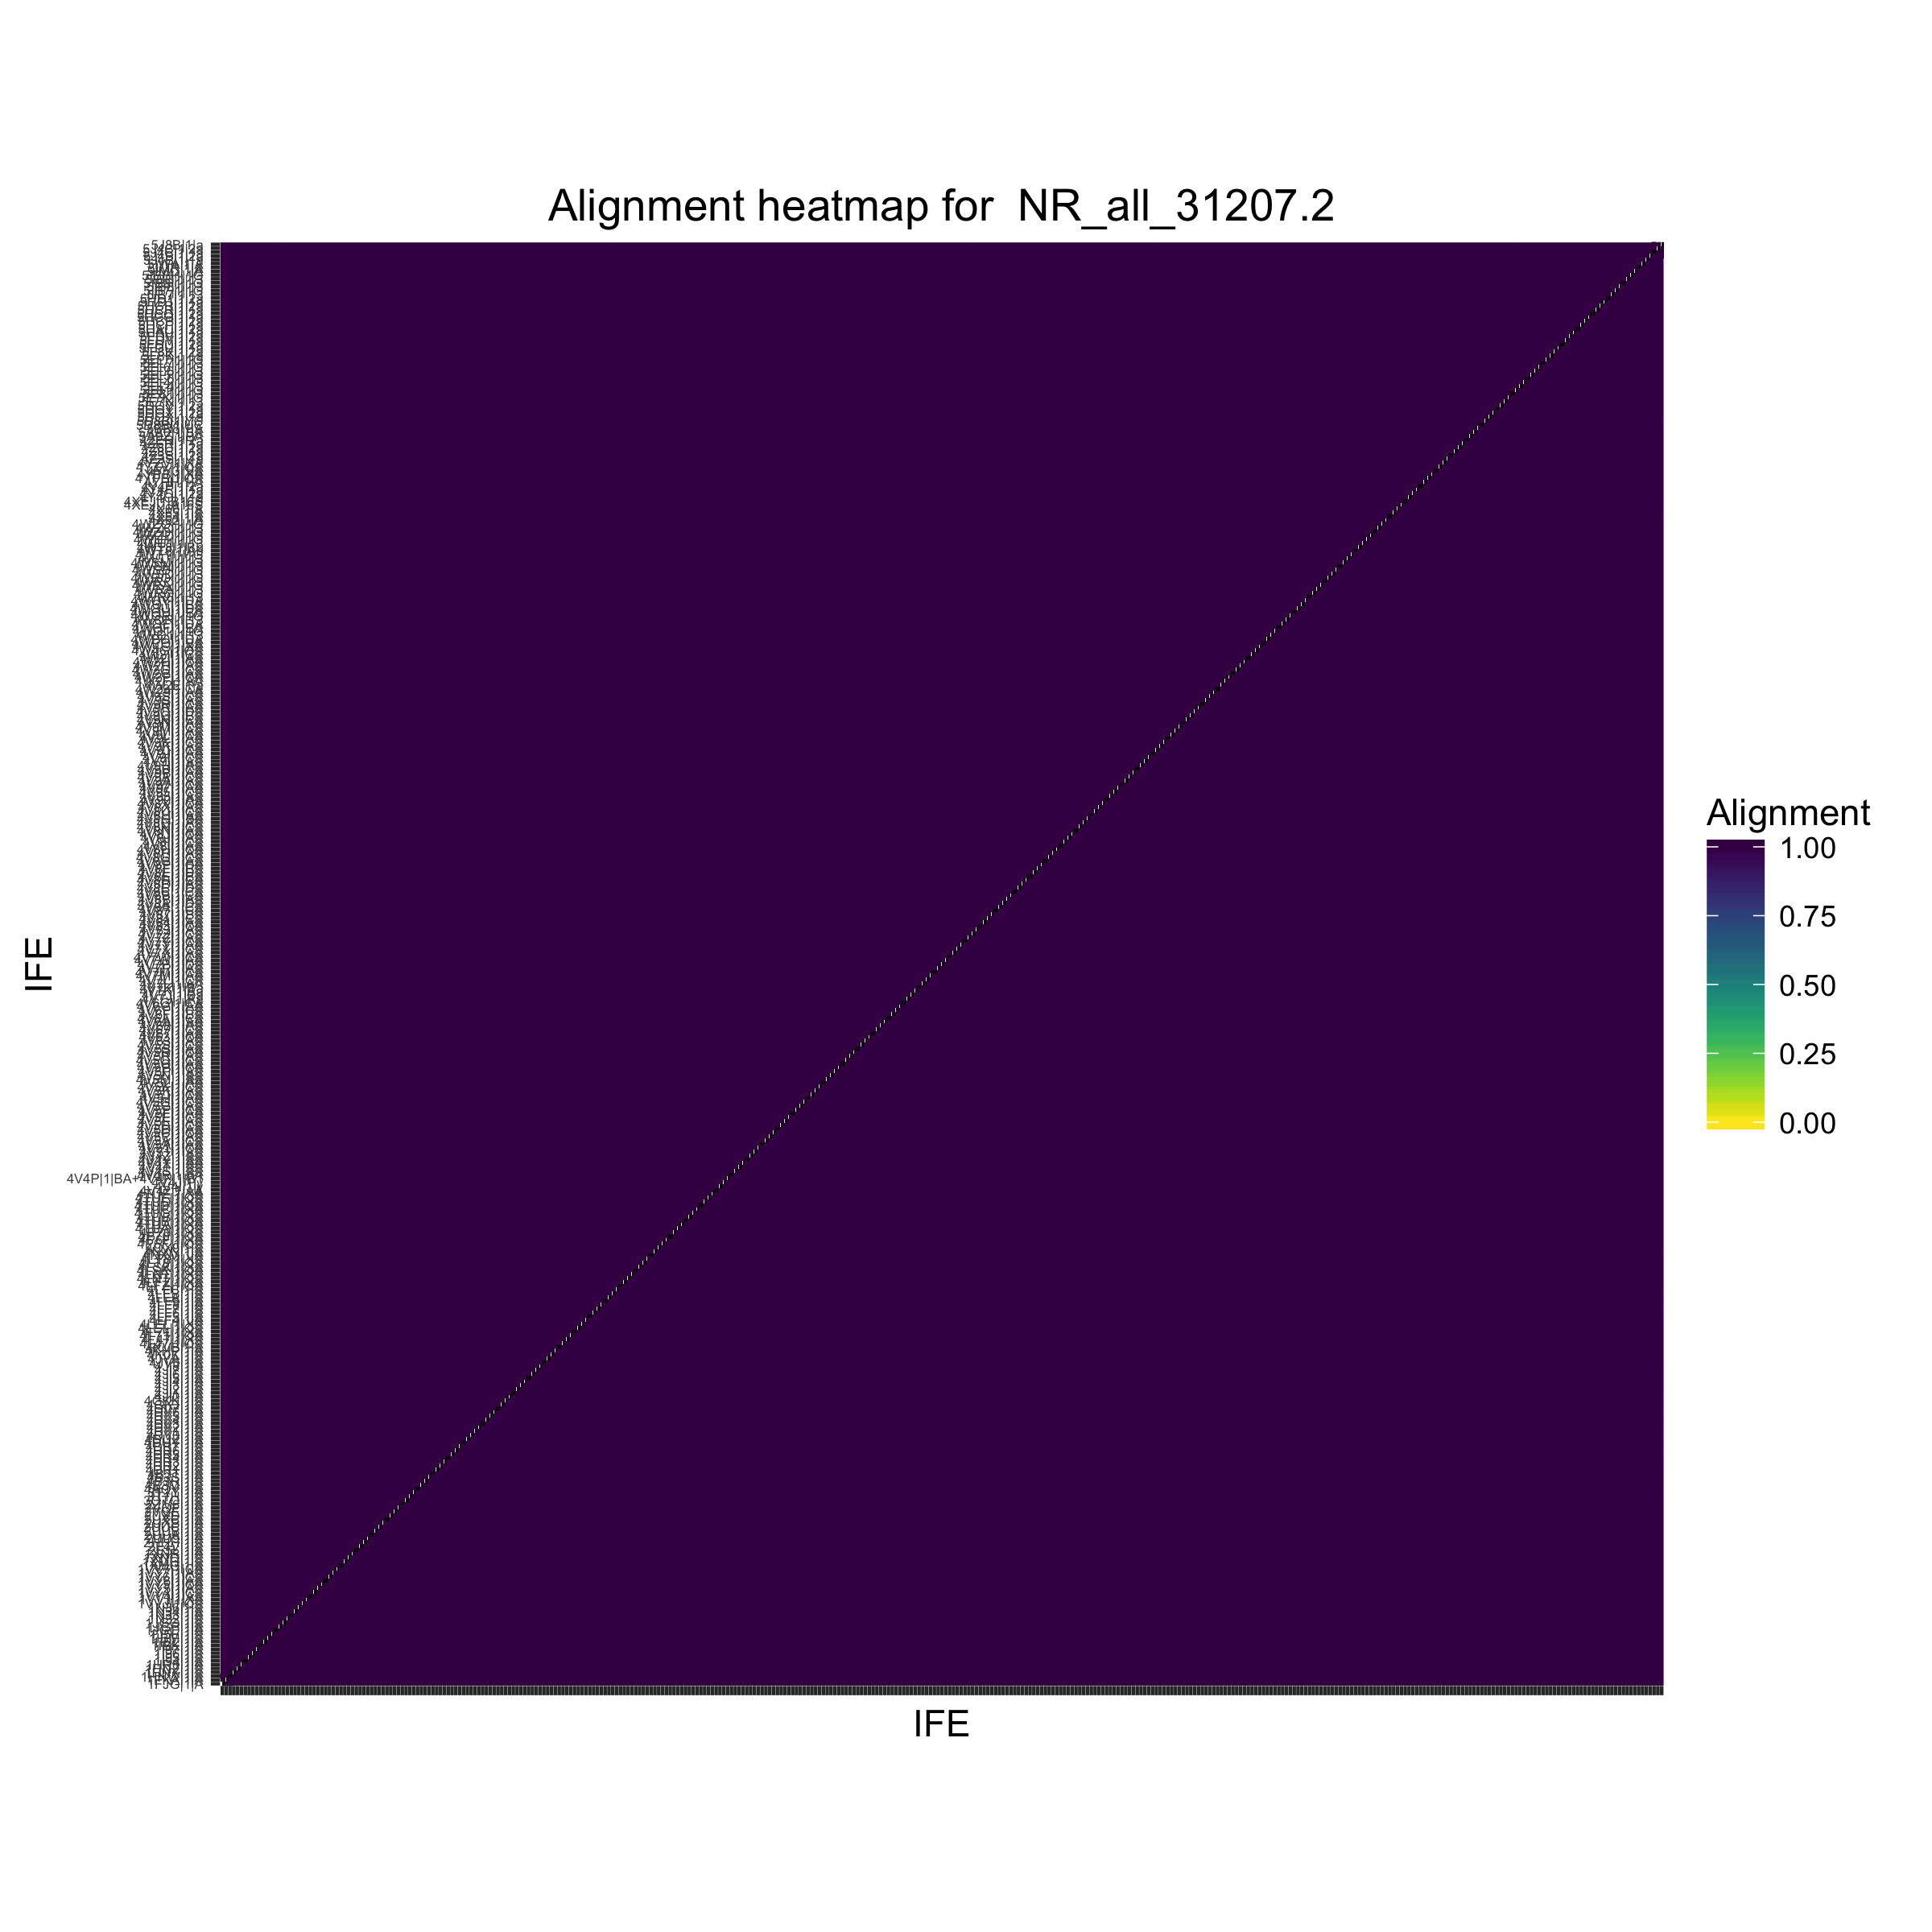
\includegraphics[width=\textwidth]{chapter-3/figs/tt-ssu-align}
  \caption{A figure summarizing the sequences similarity for all IFE's in the
    \TT{} small subunit. Color scale indicates geometric discrepancy
  values, lighter colors being worse.}
  \label{fig:tt-ssu-align}
\end{figure}

\begin{figure}[h]
  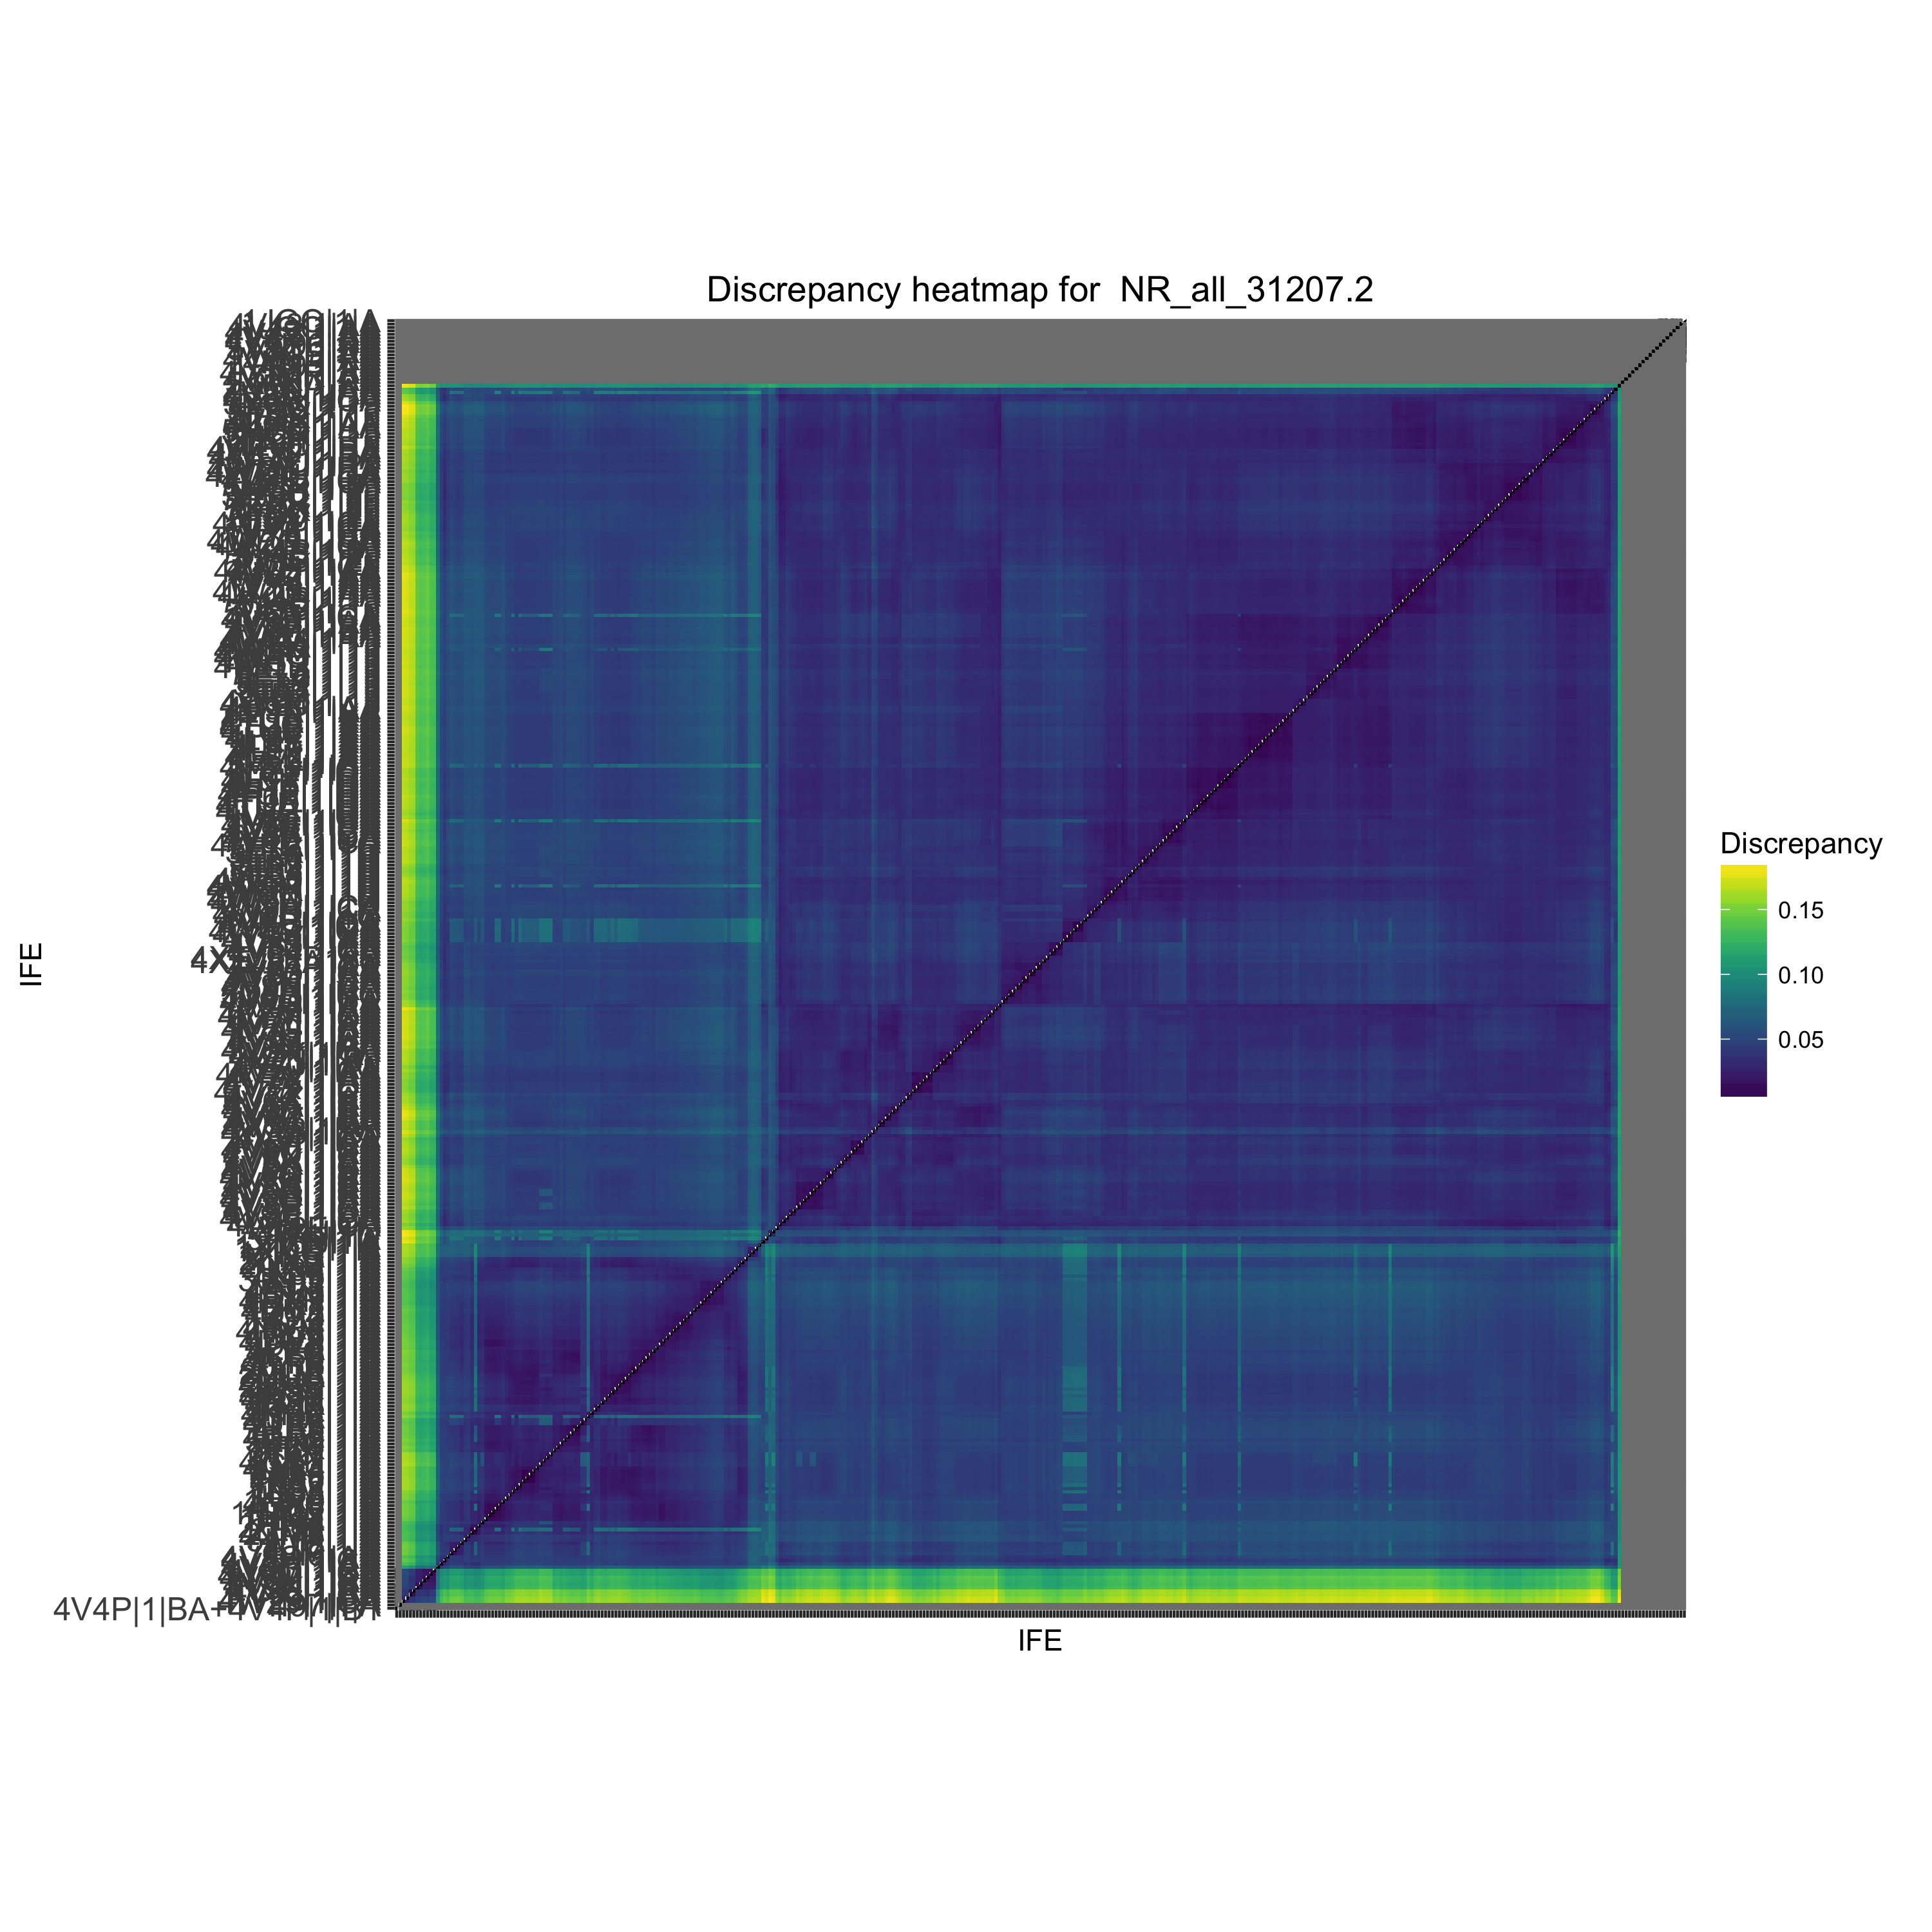
\includegraphics[width=\textwidth]{chapter-3/figs/tt-ssu-disc}
  \caption{Summary of the geometric discrepancy for all pairs of IFE's in the \TT{}
    small subunit. Grey squares indicate no data computed, because
    that structure has too low a resolution. Color scale indicates geometric discrepancy
  values, lighter colors being worse.}
  \label{fig:tt-ssu-disc}
\end{figure}

\subsection{tRNA and mRNA complexes}

We examined two classes that contained tRNA alone and tRNA/mRNA complexes. The
tRNA only group is shown in Figure~\ref{fig:trna-alone}. All IFE's in this EC
are geometrically similar and have identical sequences. However, within the EC
there are several subgroups, notably, 4WSM chains 2L and 2K are similar to each
other and geometrically distinct from all other IFE's. However, the differences
are below our cutoff of 0.4 {\AA}/nt, so they are placed the same EC.

\begin{figure}[h]
  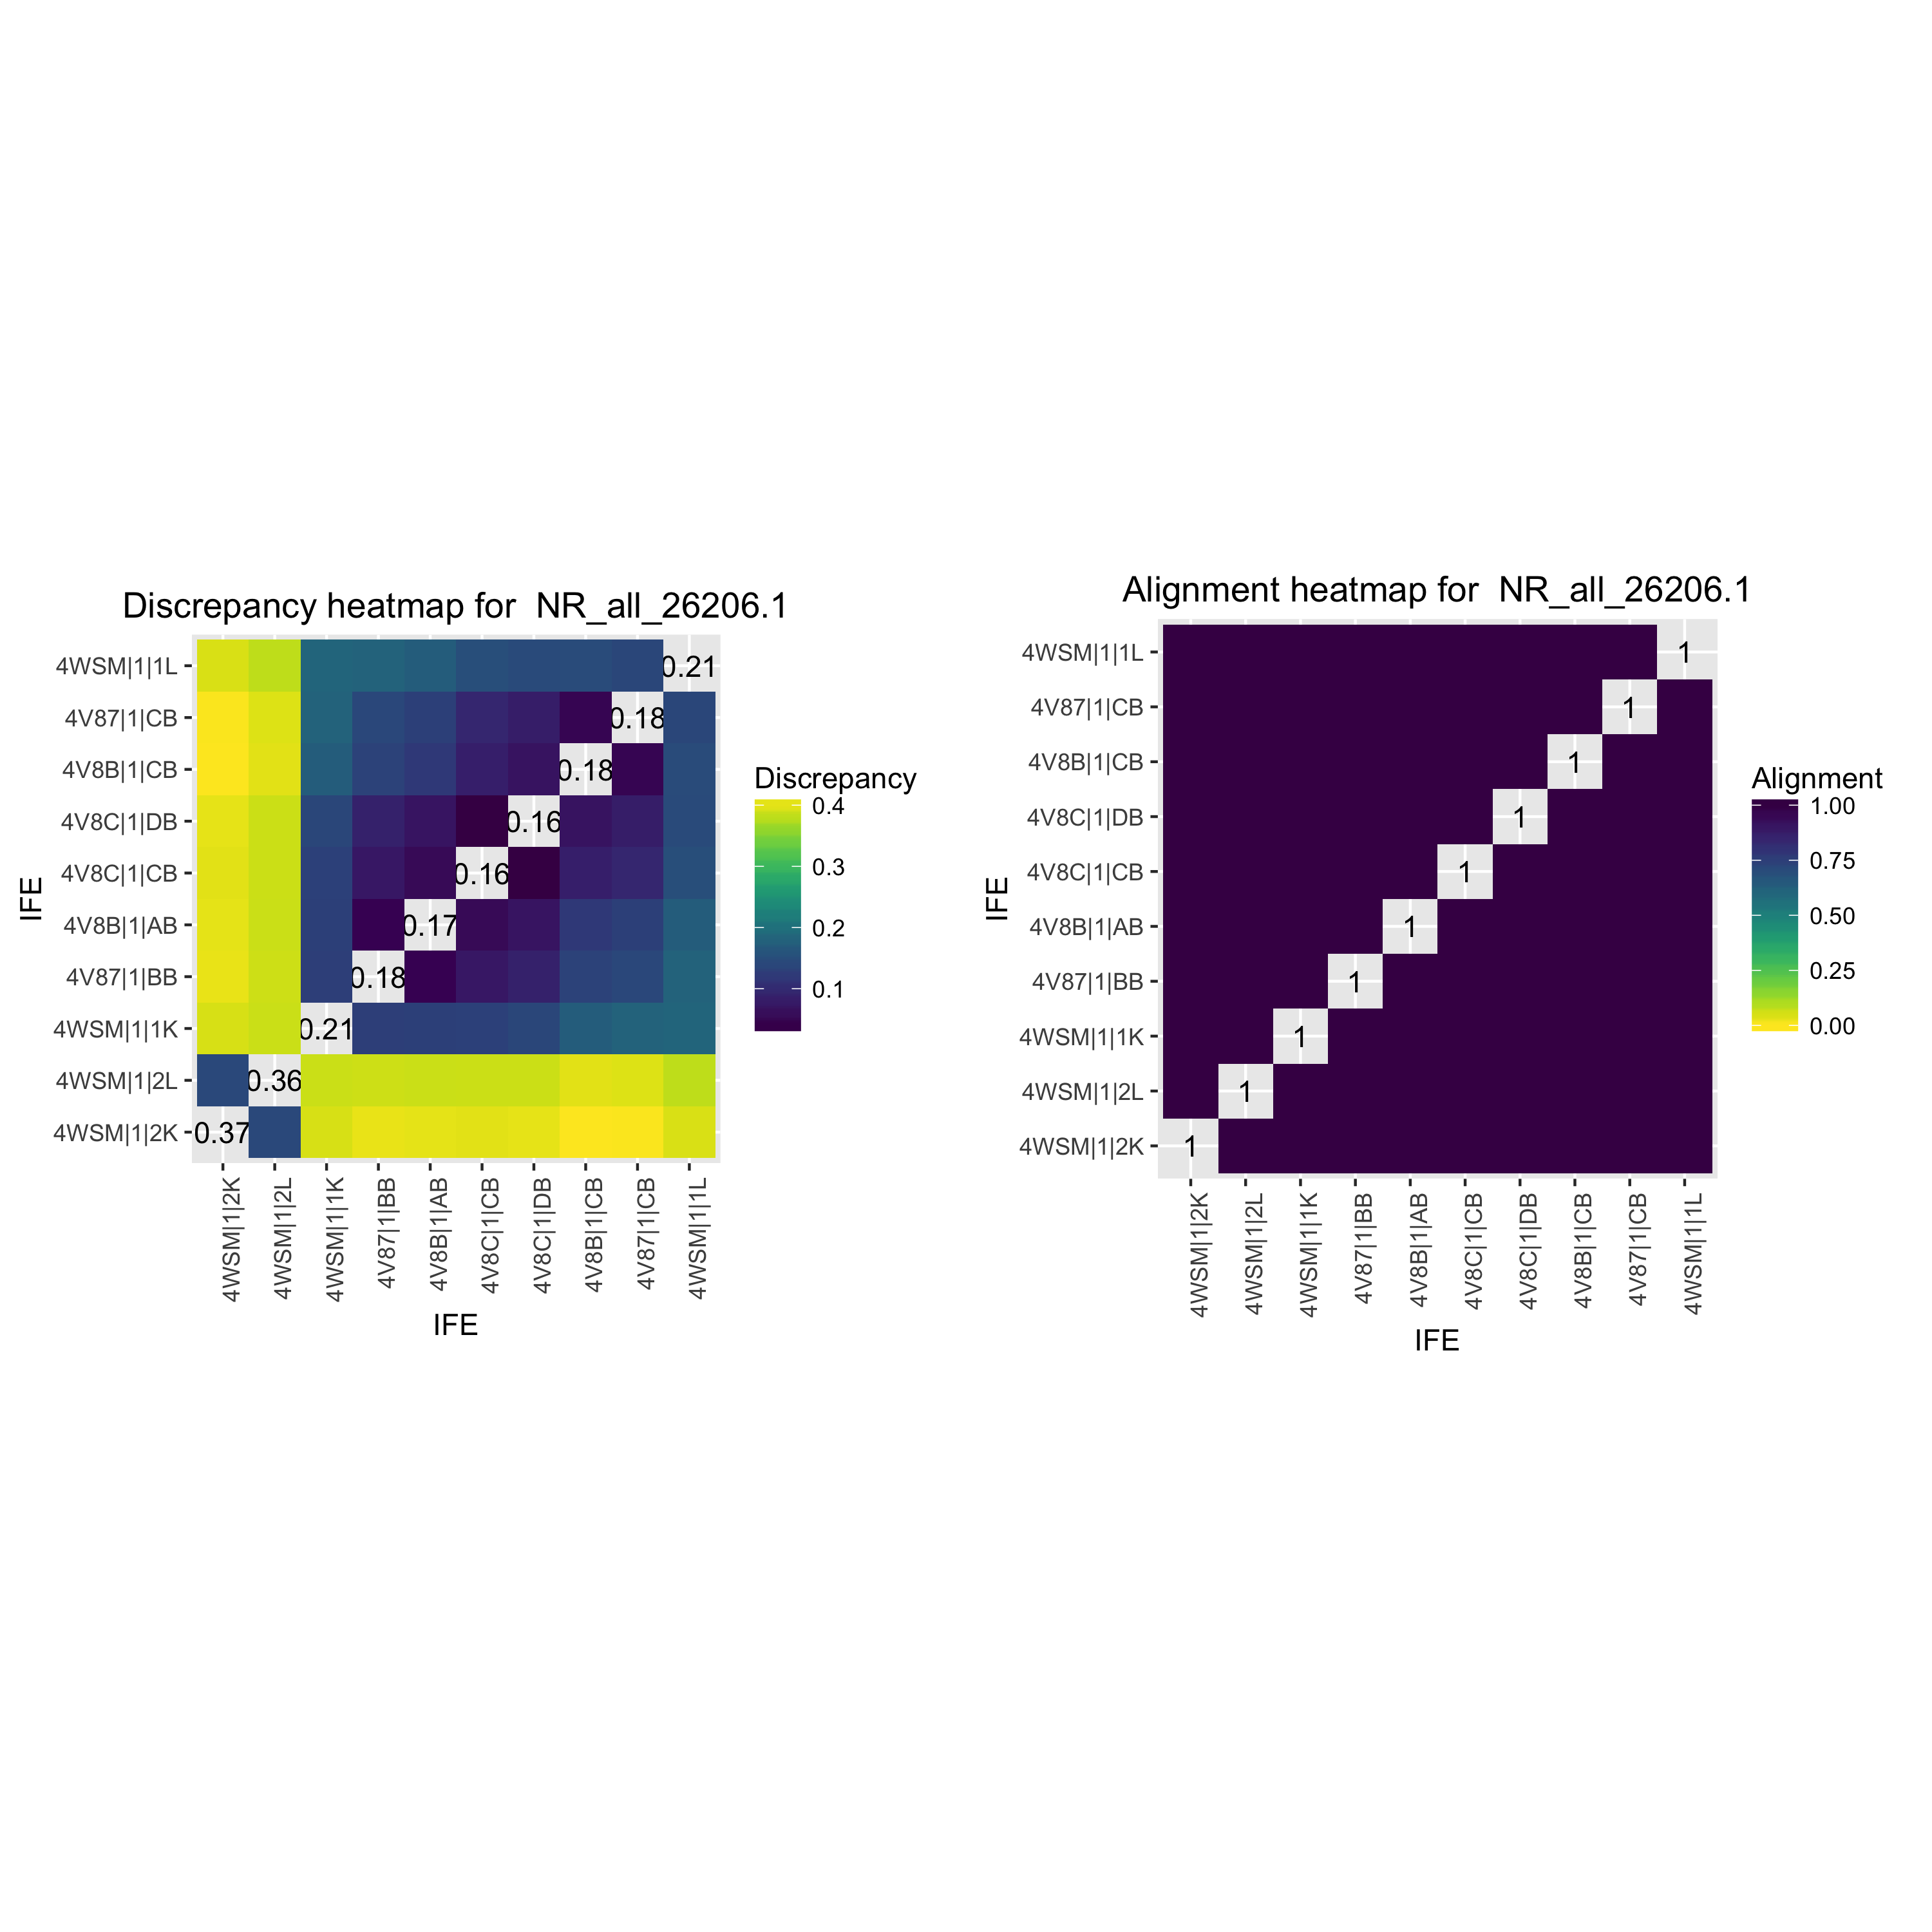
\includegraphics[width=\textwidth]{chapter-3/figs/trna-alone}
  \caption{Example of a tRNA/mRNA complex forming an equivalence class. On the
    left is a heat map of the discrepancies for all IFE's in the group. The
    right shows the heat map of sequence similarity for the group. Color scales
    indicate the value, with lighter colors meaning ``worse'' values. Along the
  diagonal of each plot is the mean value for each row.}
  \label{fig:trna-alone}
\end{figure}

\subsection{Protein and RNA complexes}

Small RNA/protein complexes are the groups which are most affected by usage of
geometric discrepancy. To test how our method works we built EC's with and
without geometric discrepancy. We used a small, 11 nt, poly-A chain as a test
case. This molecule adopts different conformations depending upon the
environment. In 4JRD it forms a non-canonical duplex, while in 1CVJ it forms a
single strand bound to a protein. Figure~\ref{fig:small-aa-no-disc} shows the
geometric discrepancy for this EC. It contains several subgroups that are only
connected by sequence, which would be separated by GD. Upon using GD this EC is
partitioned into for EC, one of which is shown in
Figure~\ref{fig:small-aa-disc}. In this heatmap we can see that the smaller EC
is much more homogeneous, with all pairs have geometric discrepancy less than
0.2{\AA}/nt. In addition all members of this EC form similar structures that are
bound to proteins, unlike the previous method which produced EC's that mixed
together single and double stranded molecules.

\begin{figure}[h]
  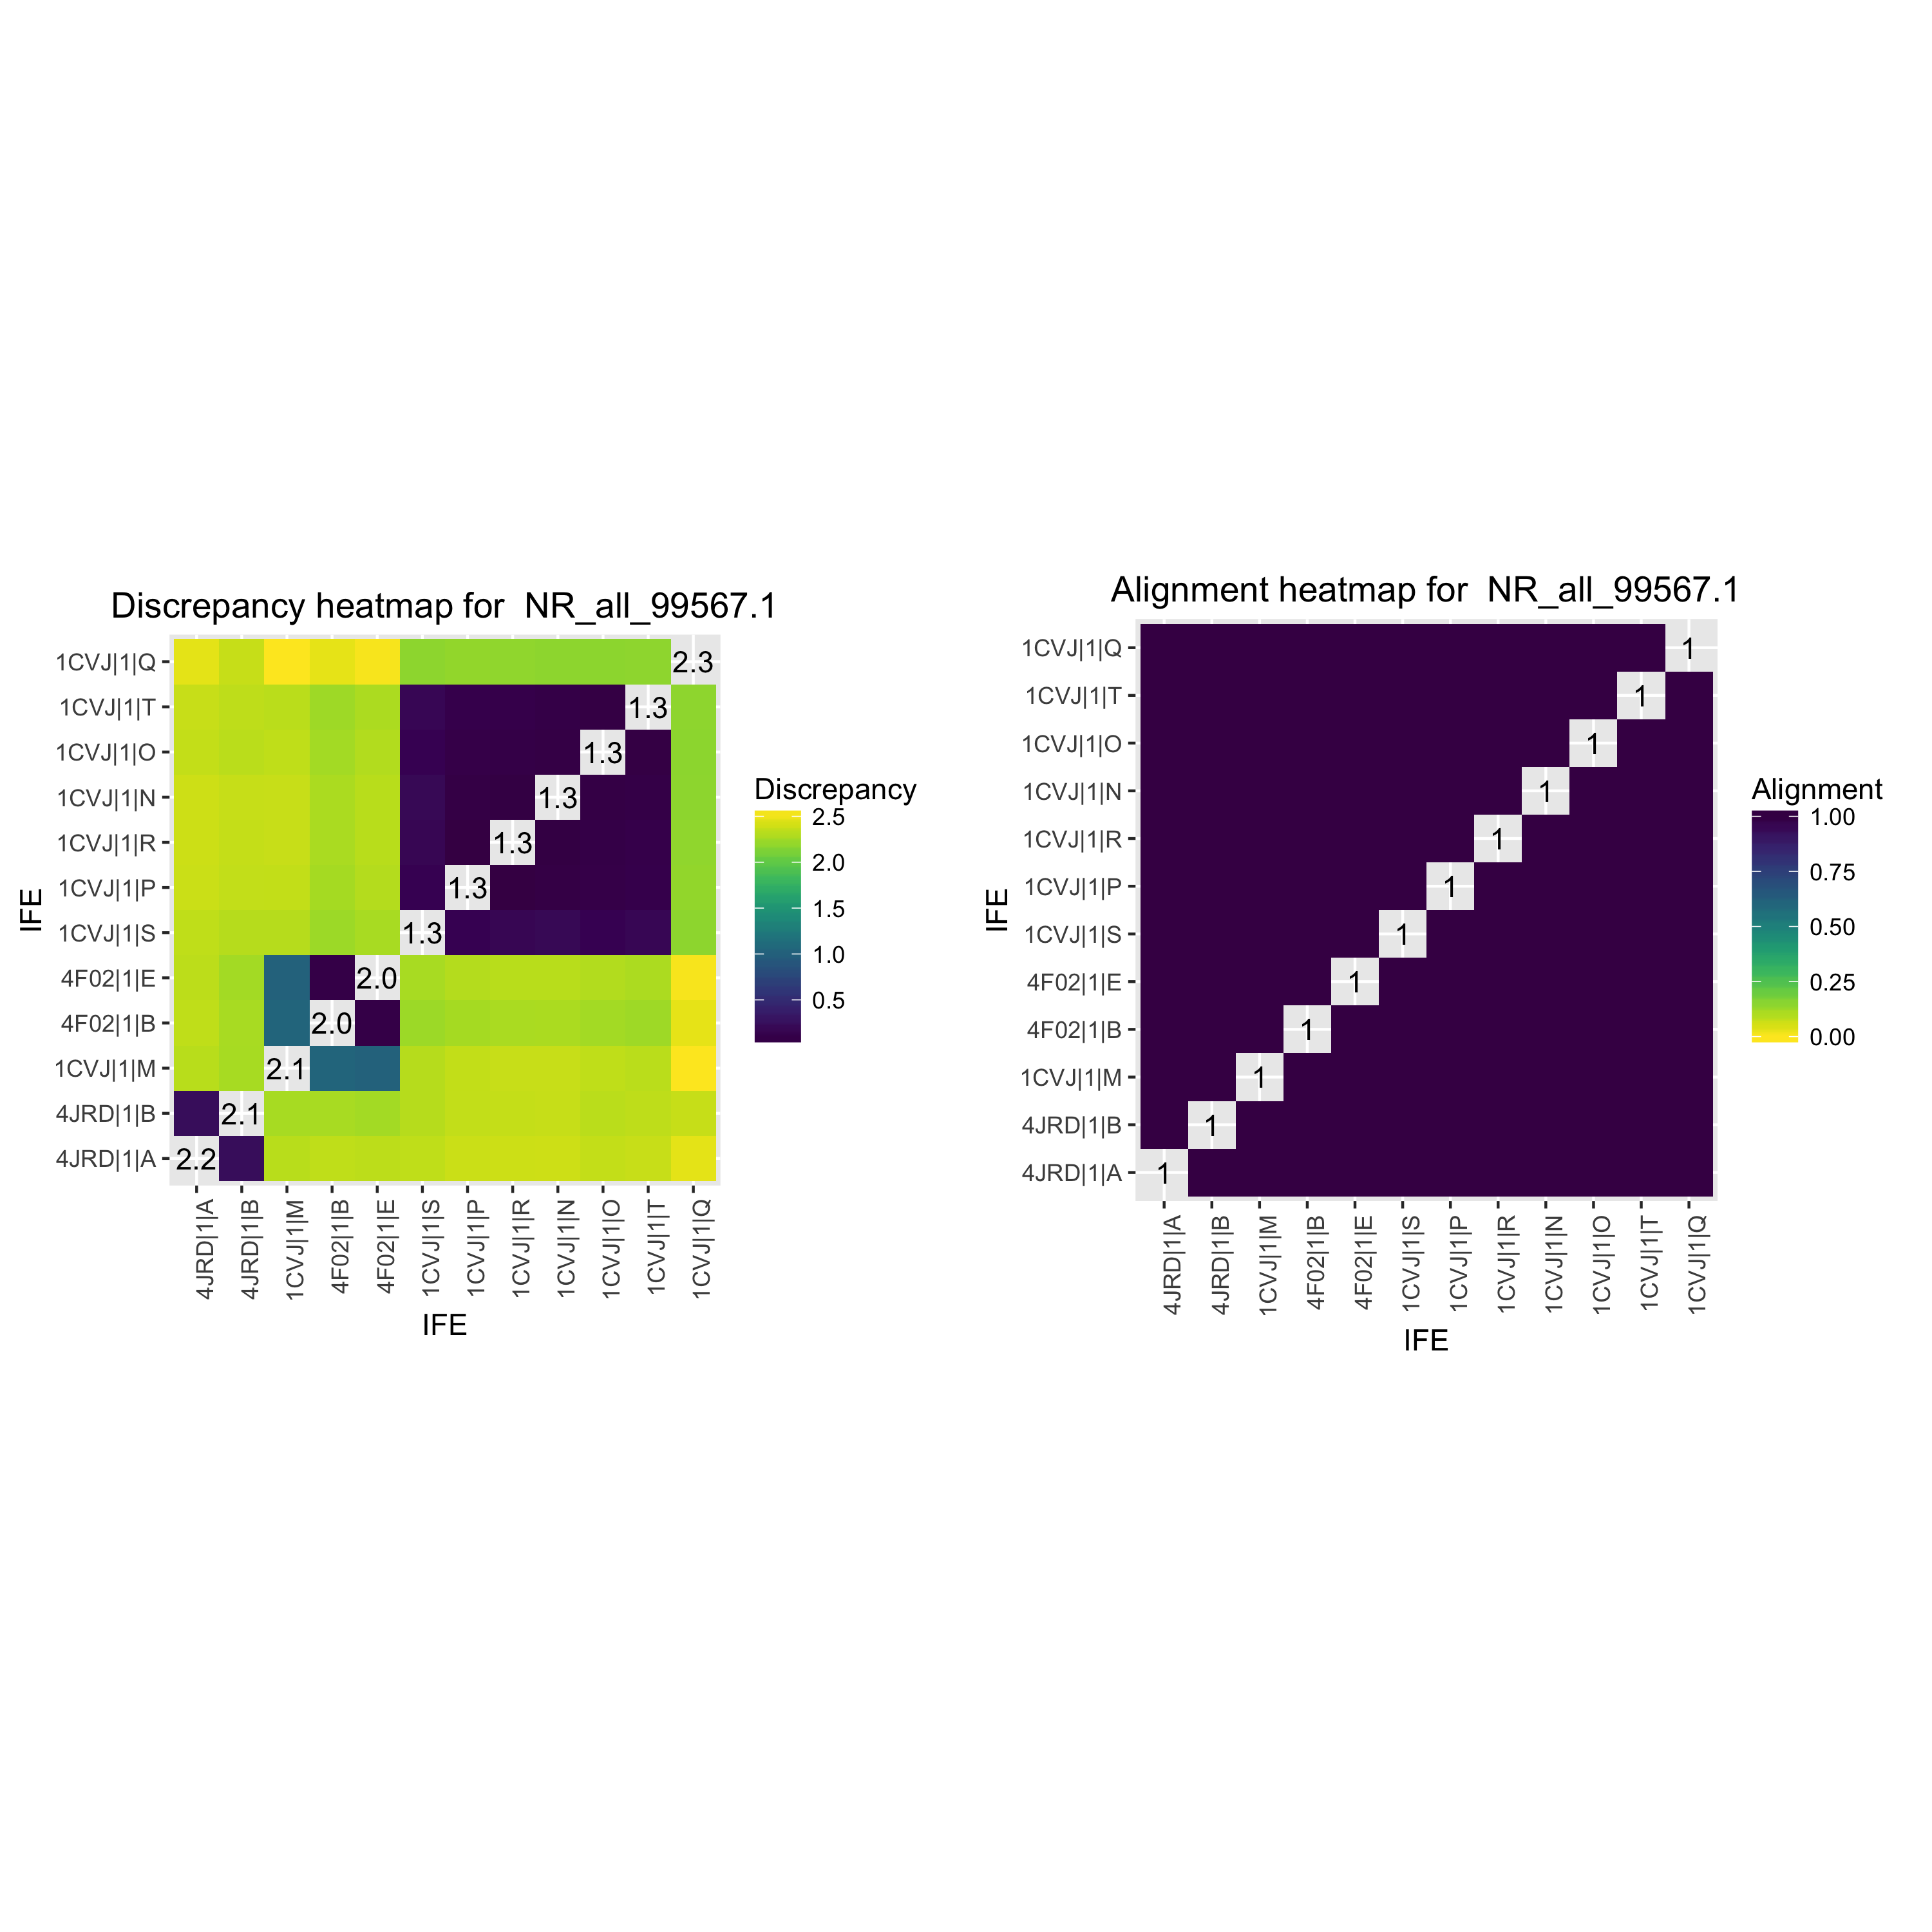
\includegraphics[width=\textwidth]{chapter-3/figs/small-aa-no-disc}
  \caption{geometric discrepancy heatmap for an 11-nt poly-A class built without
    geometric discrepancy: This shows the effect of clustering a model compound without
    using geometric discrepancy. We are showing only the geometric discrepancy heatmap here. We can
  see that there are several subgroups with very different geometries.}
  \label{fig:small-aa-no-disc}
\end{figure}

\begin{figure}[h]
  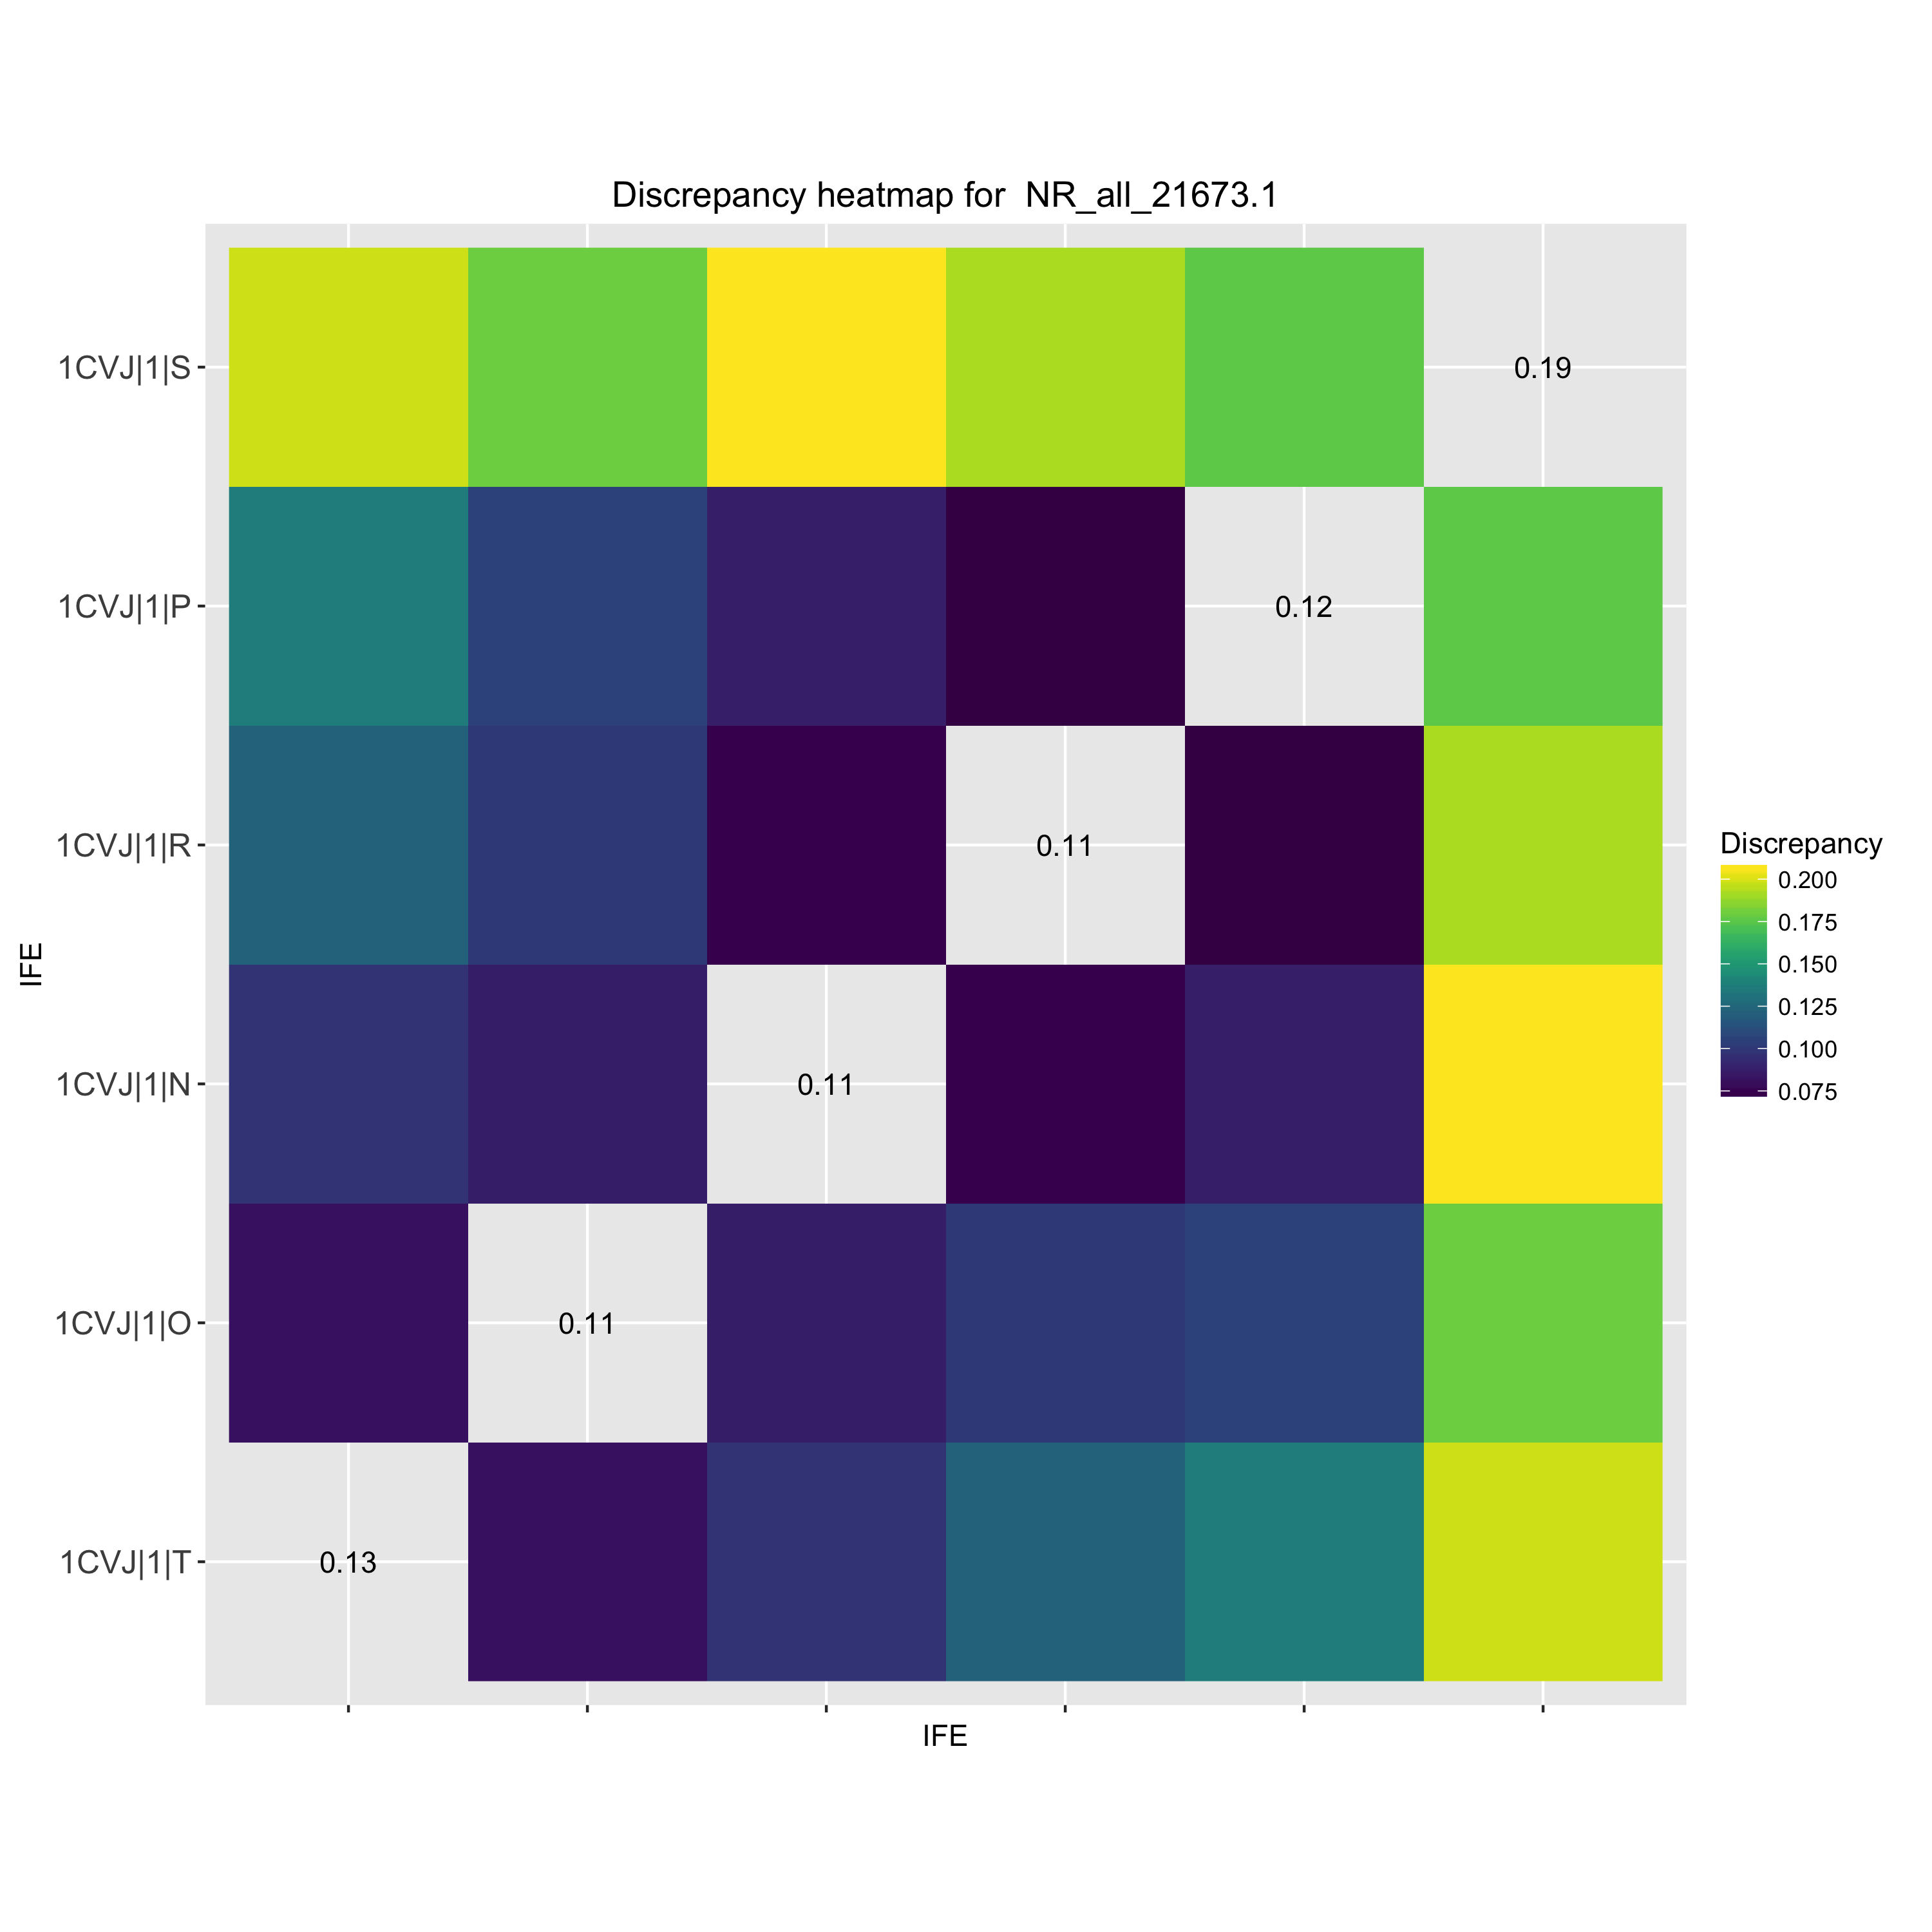
\includegraphics[width=\textwidth]{chapter-3/figs/small-aa-disc}
  \caption{geometric discrepancy heatmap for a small 11-nt poly-A compound built using
    geometric discrepancy. Mean values for each row are shown on the diagonal, and the
  color scale indicates geometric discrepancy with lighter colors being worse}
  \label{fig:small-aa-disc}
\end{figure}

\subsection{Outliers}

After evaluating specific cases we searched for outliers within EC's. I began by
examining the distribution of maximum geometric discrepancy and minimum sequence
similarity for all pairs in all equivalence classes. Figure~\ref{fig:eq-summary}
shows that most groups have a low geometric discrepancy and high sequence
similarity. However, there is a very long tail of groups with high
discrepancies, some even ranging up to 4{\AA}/nt. This indicates that some EC's
contain pairs of IFE's that are highly dissimilar. For the purpose of this
analysis I define EC's with outliers as EC's that contain one or more pairs of
IFE's with GD greater than 0.8{\AA}/nt or any EC that contains a pair of IFE's
that do not meet the sequence similarity criterion. As discussed earlier, our
criterion for sequence similarity depends on the size of the chains. For this
reason we cannot use a simple sequence similarity cutoff as with GD.

\begin{figure}[h]
  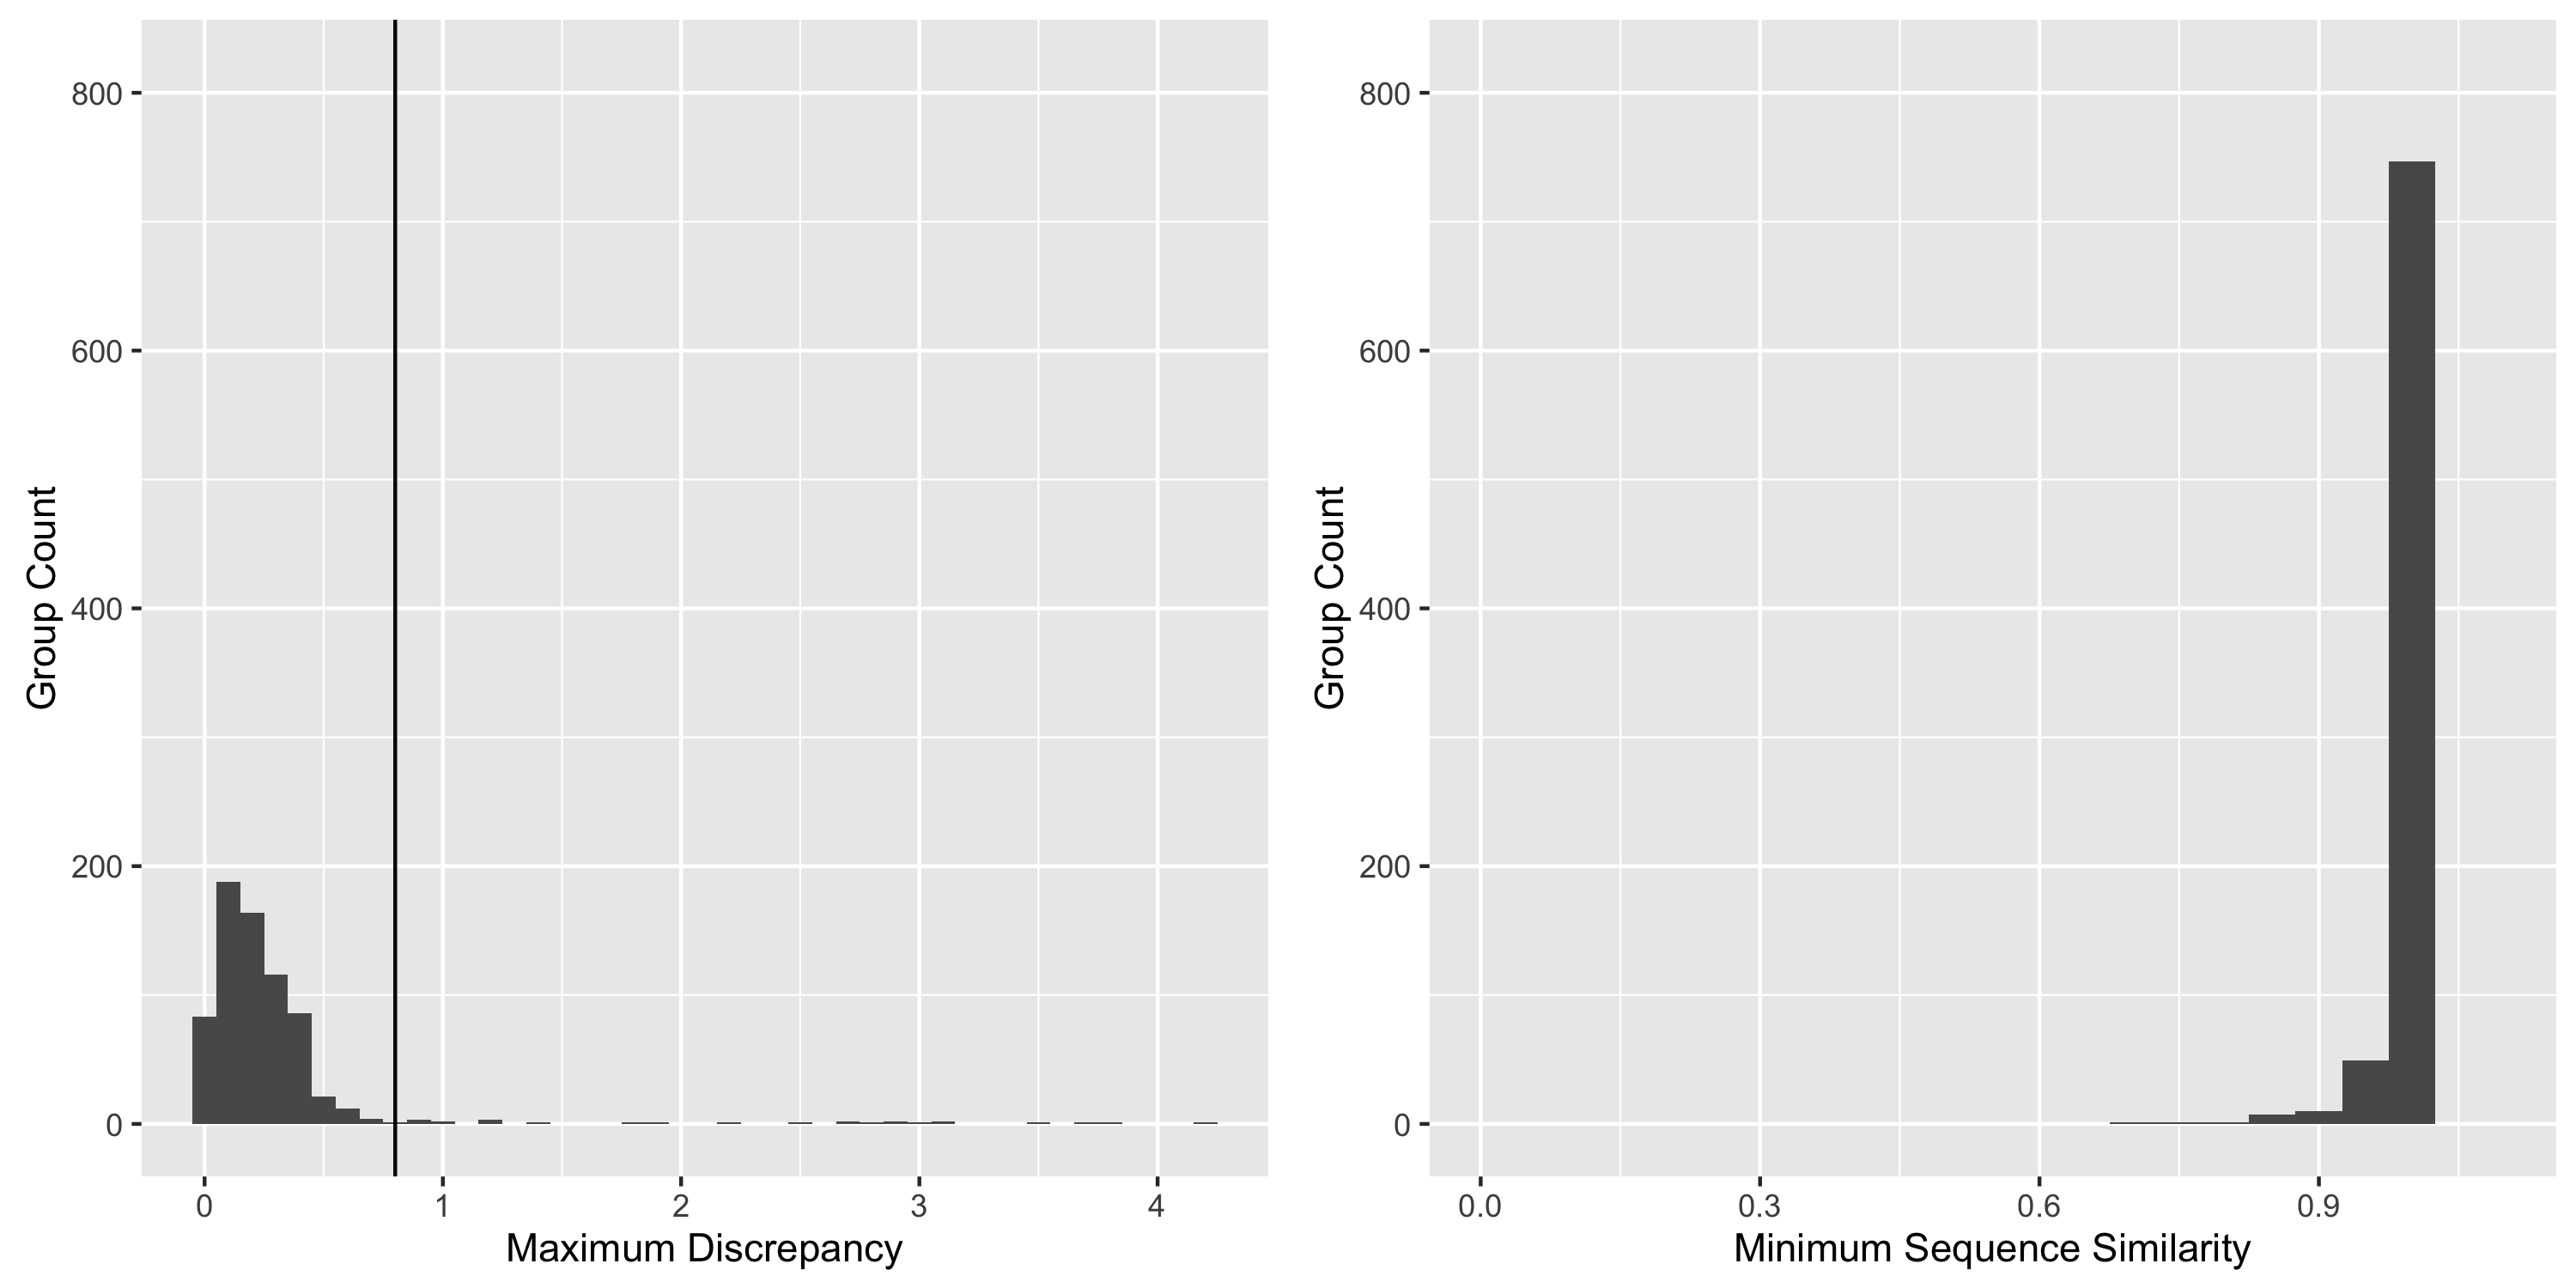
\includegraphics[width=\textwidth]{chapter-3/figs/eq-summary}
  \caption{A figure of the Maximum Pairwise geometric discrepancy and Minimum Sequence
    Similarity for all pairs of IFE's in all equivalence classes. The black
    lines indicate the 0.8 geometric discrepancy cutoff (left) used a criterion for
  detecting groups with outlier pairs.}
  \label{fig:eq-summary}
\end{figure}

I then investigated the distribution of GD and sequence similarities for all
groups containing outliers. These data are plotted in
Figure~\ref{fig:eq-outlier-summary}. This graph shows that outliers appear in
all regions of the graph. Some outliers have low geometric discrepancy,
indicating they differ in sequence, while others have high sequence similarity
indicating they differ geometrically.

\begin{figure}[h]
  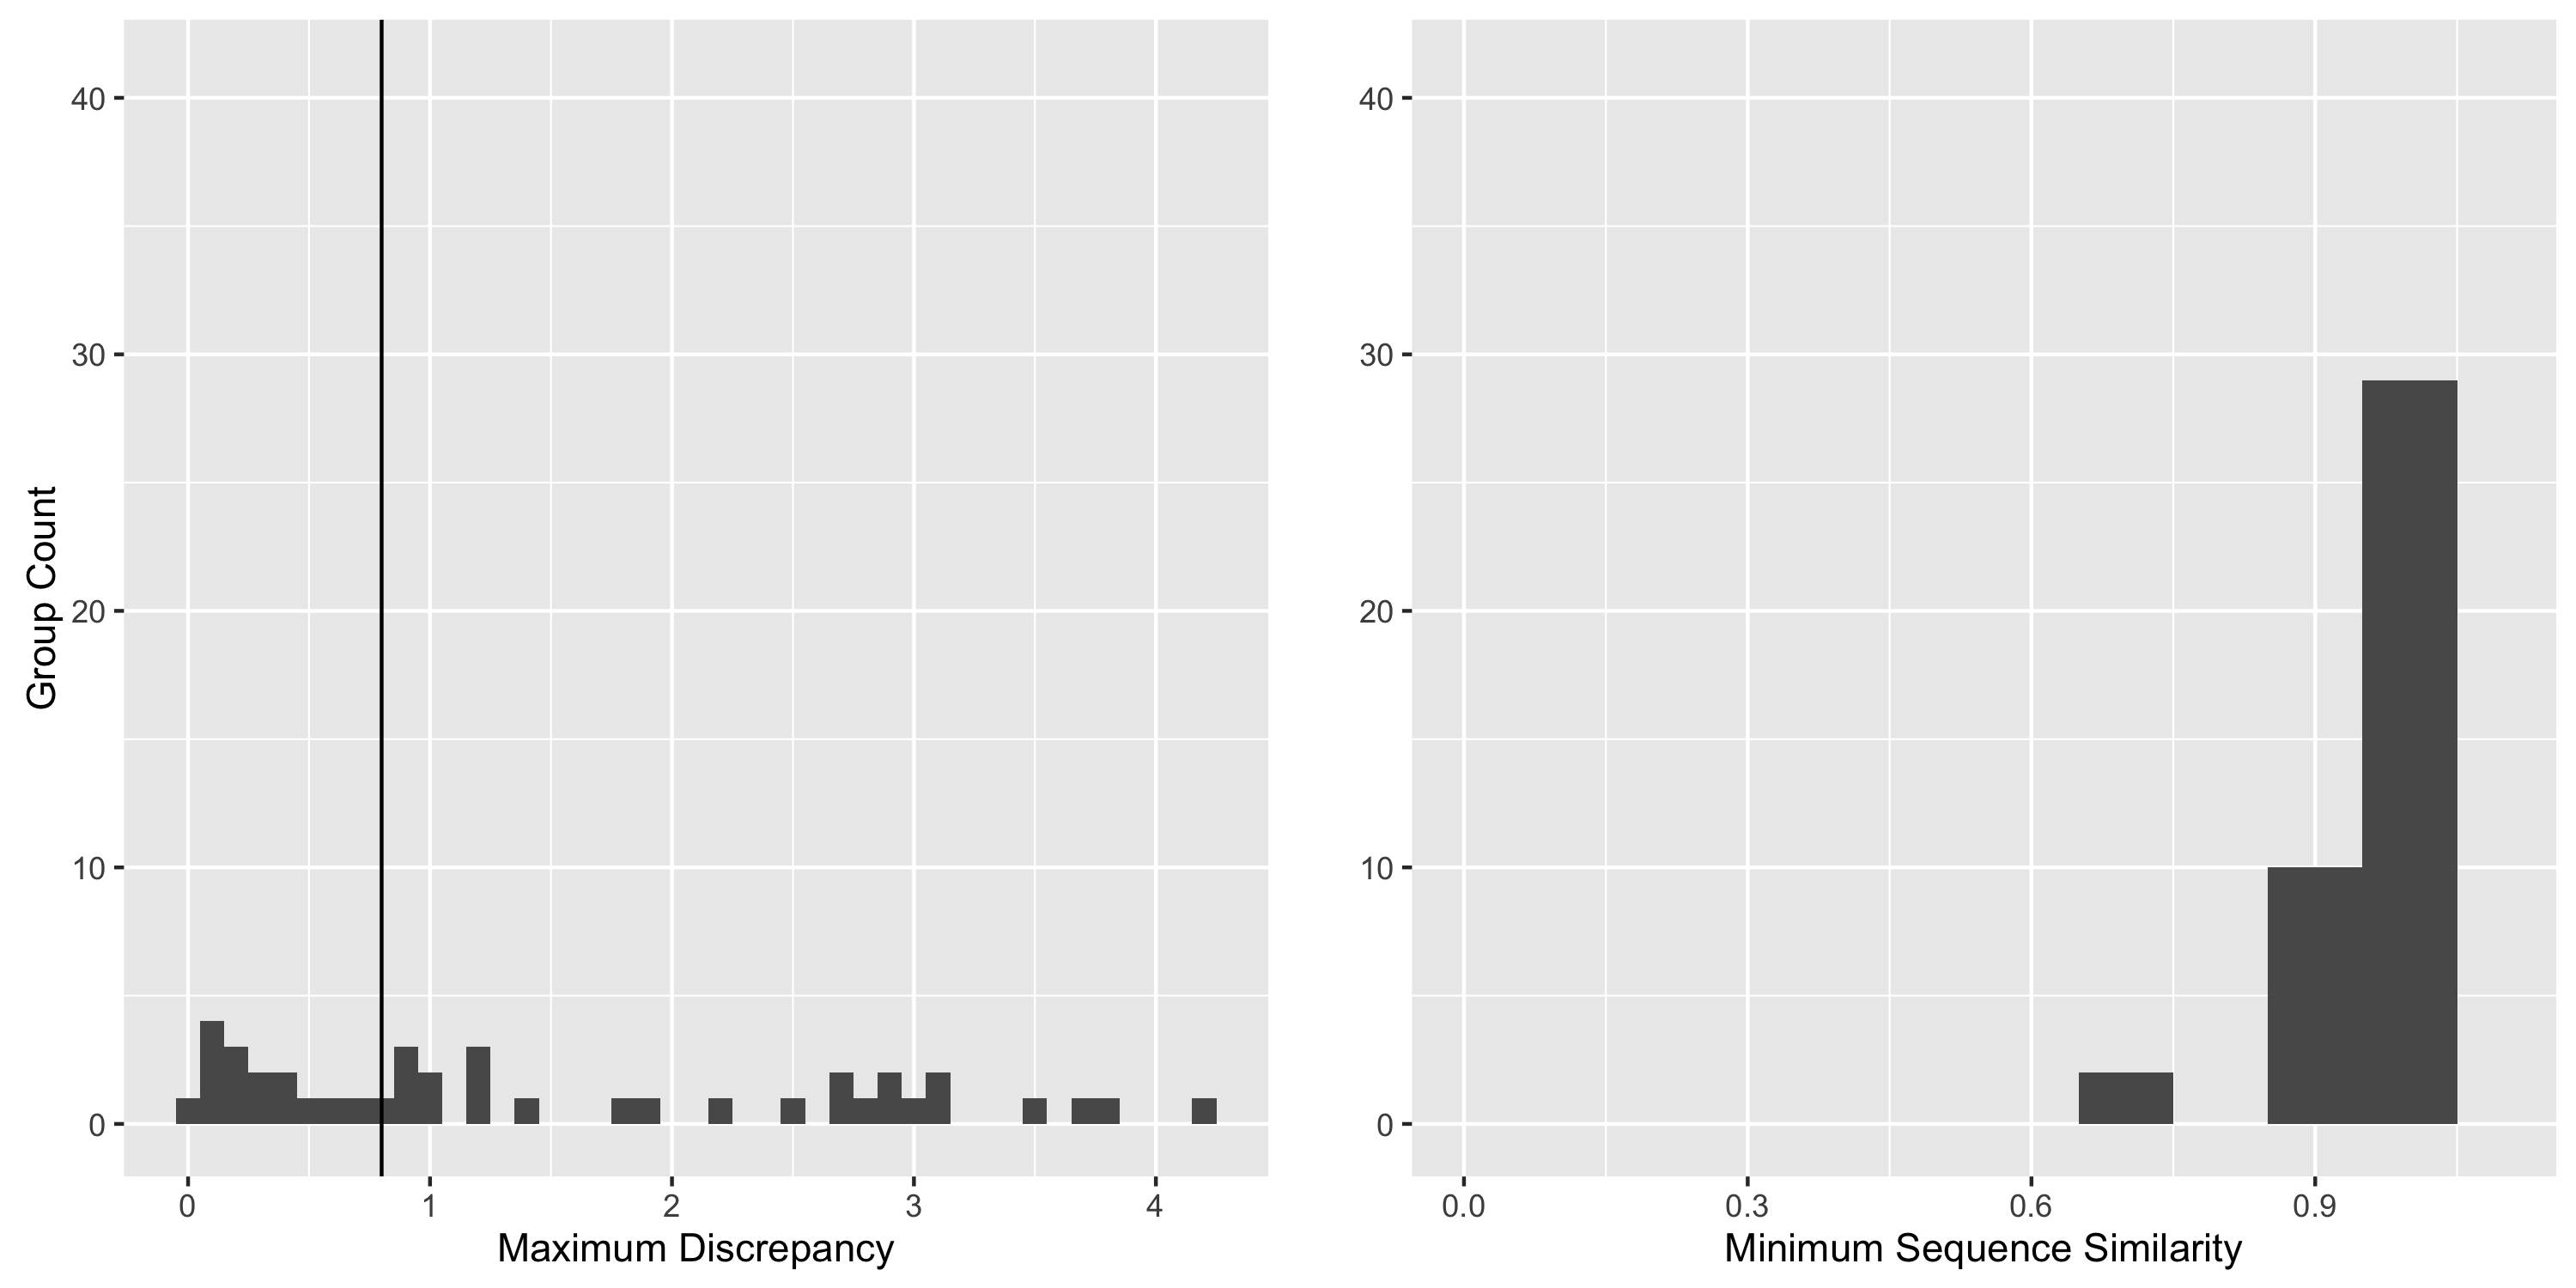
\includegraphics[width=\textwidth]{chapter-3/figs/outlier-summary}
  \caption{geometric discrepancy and Minimum Sequence Similarity of all groups with
  outliers. This figure shows the same data as Figure~\ref{fig:eq-summary} but
only for groups that have a pair of IFE's with geometric discrepancy at least 0.8 or
sequence similarity less than or equal to 0.9.}
  \label{fig:eq-outlier-summary}
\end{figure}

We next examined the distribution of the number of outliers, fraction of
outliers, geometric discrepancy, and sequence similarity with respect to the
size of the group in terms of nucleotides and members as shown in
Figure~\ref{fig:outlier-detail}. This figure shows that the majority of the EC's
with outliers contain relatively few IFE's and are relatively small. However,
there are a few groups that contain many IFE's. The spike at \TILDE 80
nucleotides corresponds to two tRNA groups.

\begin{figure}[h]
  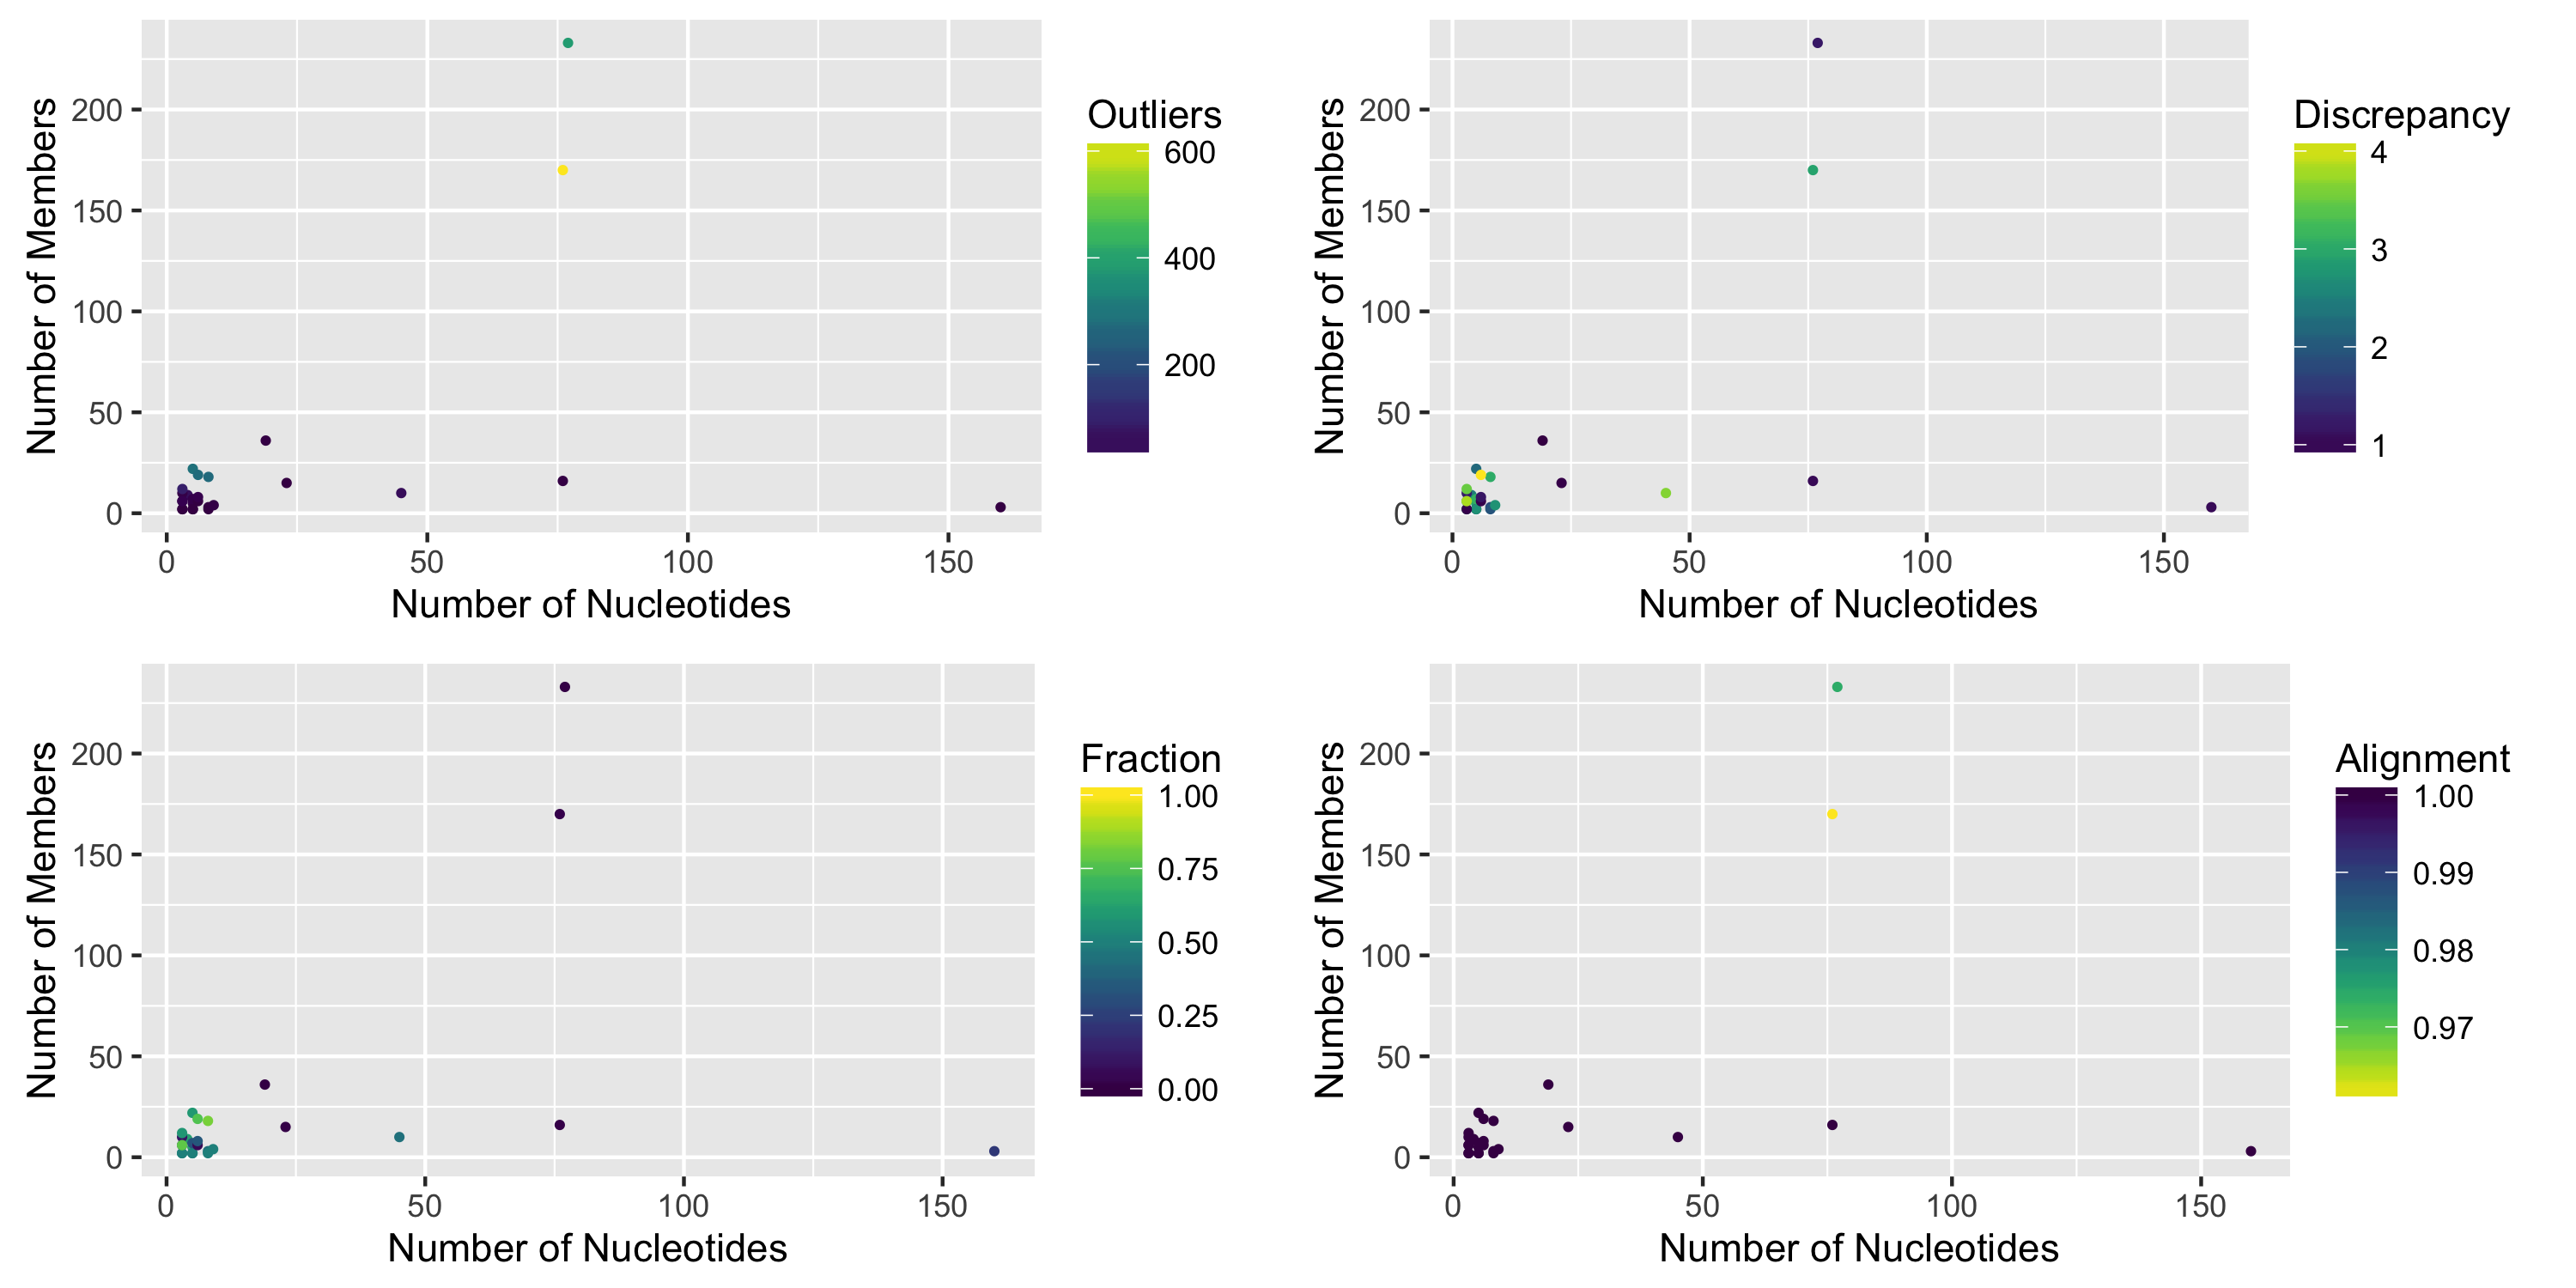
\includegraphics[width=\textwidth]{chapter-3/figs/outlier-details}
  \caption{This figure shows 4 different metrics for outliers within each group.
    Each point in all graphs represents a group that contains at least one pair
    of IFE's that is an outlier (geometric discrepancy greater than 0.8 or sequence
    similarity less than 0.9). In all graphs the horizontal coordinate is the
    number of nucleotides in the representative (discussed in the next chapter)
    of the group. The vertical is the number of members. The points are colored
    according to various metrics. In the upper right the points are colored
    using the number of pairs that are outliers, with lighter colors meaning
    more. Proceeding clockwise to the upper right the points are colored
    according to the maximum geometric discrepancy amongst all pairs in the groups.
    The lower right shows the minimum sequence similarity with lighter being a
    lower (worse) score. Finally, the lower left colors the points using the
    fraction of total pairs that are outliers, with lighter being higher
  fraction and thus worse.}
  \label{fig:outlier-detail}
\end{figure}

All EC with outliers can be classified according to the type of outliers they
contain. The EC may contain pairs of IFE's that have only high geometric
discrepancy, or only low sequence similarity or both high geometric discrepancy
and low sequence similarity. I determined the counts for each of these as shown
in Table~\ref{tab:outlier-types}, which shows that the majority of the groups,
63\%, have at least one pair with high geometric discrepancy. The remaining 36\%
of groups contain pairs that have low sequence similarity and no pairs with high
geometric discrepancy. I explored these classes to determine how such EC were
built.

\begin{table}
  \begin{tabular}{lr}
    \toprule
    Outlier Type & Number of Groups (Percent) \\
    \midrule
    High geometric discrepancy & 21 (51\%) \\
    Low Sequence Similarity & 15 (36\%) \\
    High geometric discrepancy and Low Sequence Similarity & 5 (12\%) \\
    \bottomrule
  \end{tabular}
  \caption{This table shows the counts, and percents, of each type of outlier
  in an equivalence class.}
  \label{tab:outlier-types}
\end{table}

From the definition of our methodology, I know that all EC that contain pairs
with low sequence similarity will do so because they are connected through a
transitive chain of high sequence similarity pairs. For example, the
NR\_all\_03381.1 group contains protein/stem loop constructs of length 22 nt and
has 4 members, \ife{1K8W}{1}{B}, \ife{1ZL3}{1}{B}, \ife{1ZE2}{1}{D}, and
\ife{1ZE2}{1}{C}.

The other class of EC with outliers, those that contain a pair with high
geometric discrepancy, can be caused in two ways. First, the pairs may be
connected through a transitive chain of low discrepancies, similar to pairs with
low sequence similarity being connected through a chain of high sequence
similarity pairs. This is visible in Figure~\ref{fig:nr-all-75770.1-disc}. In
this figure there are yellow bars that are not as long as the entire plot. This
means that the IFE is dissimilar to some other IFE's but similar to others,
indicating it is connected through a transitive chain of low similarity.

\begin{figure}[h]
  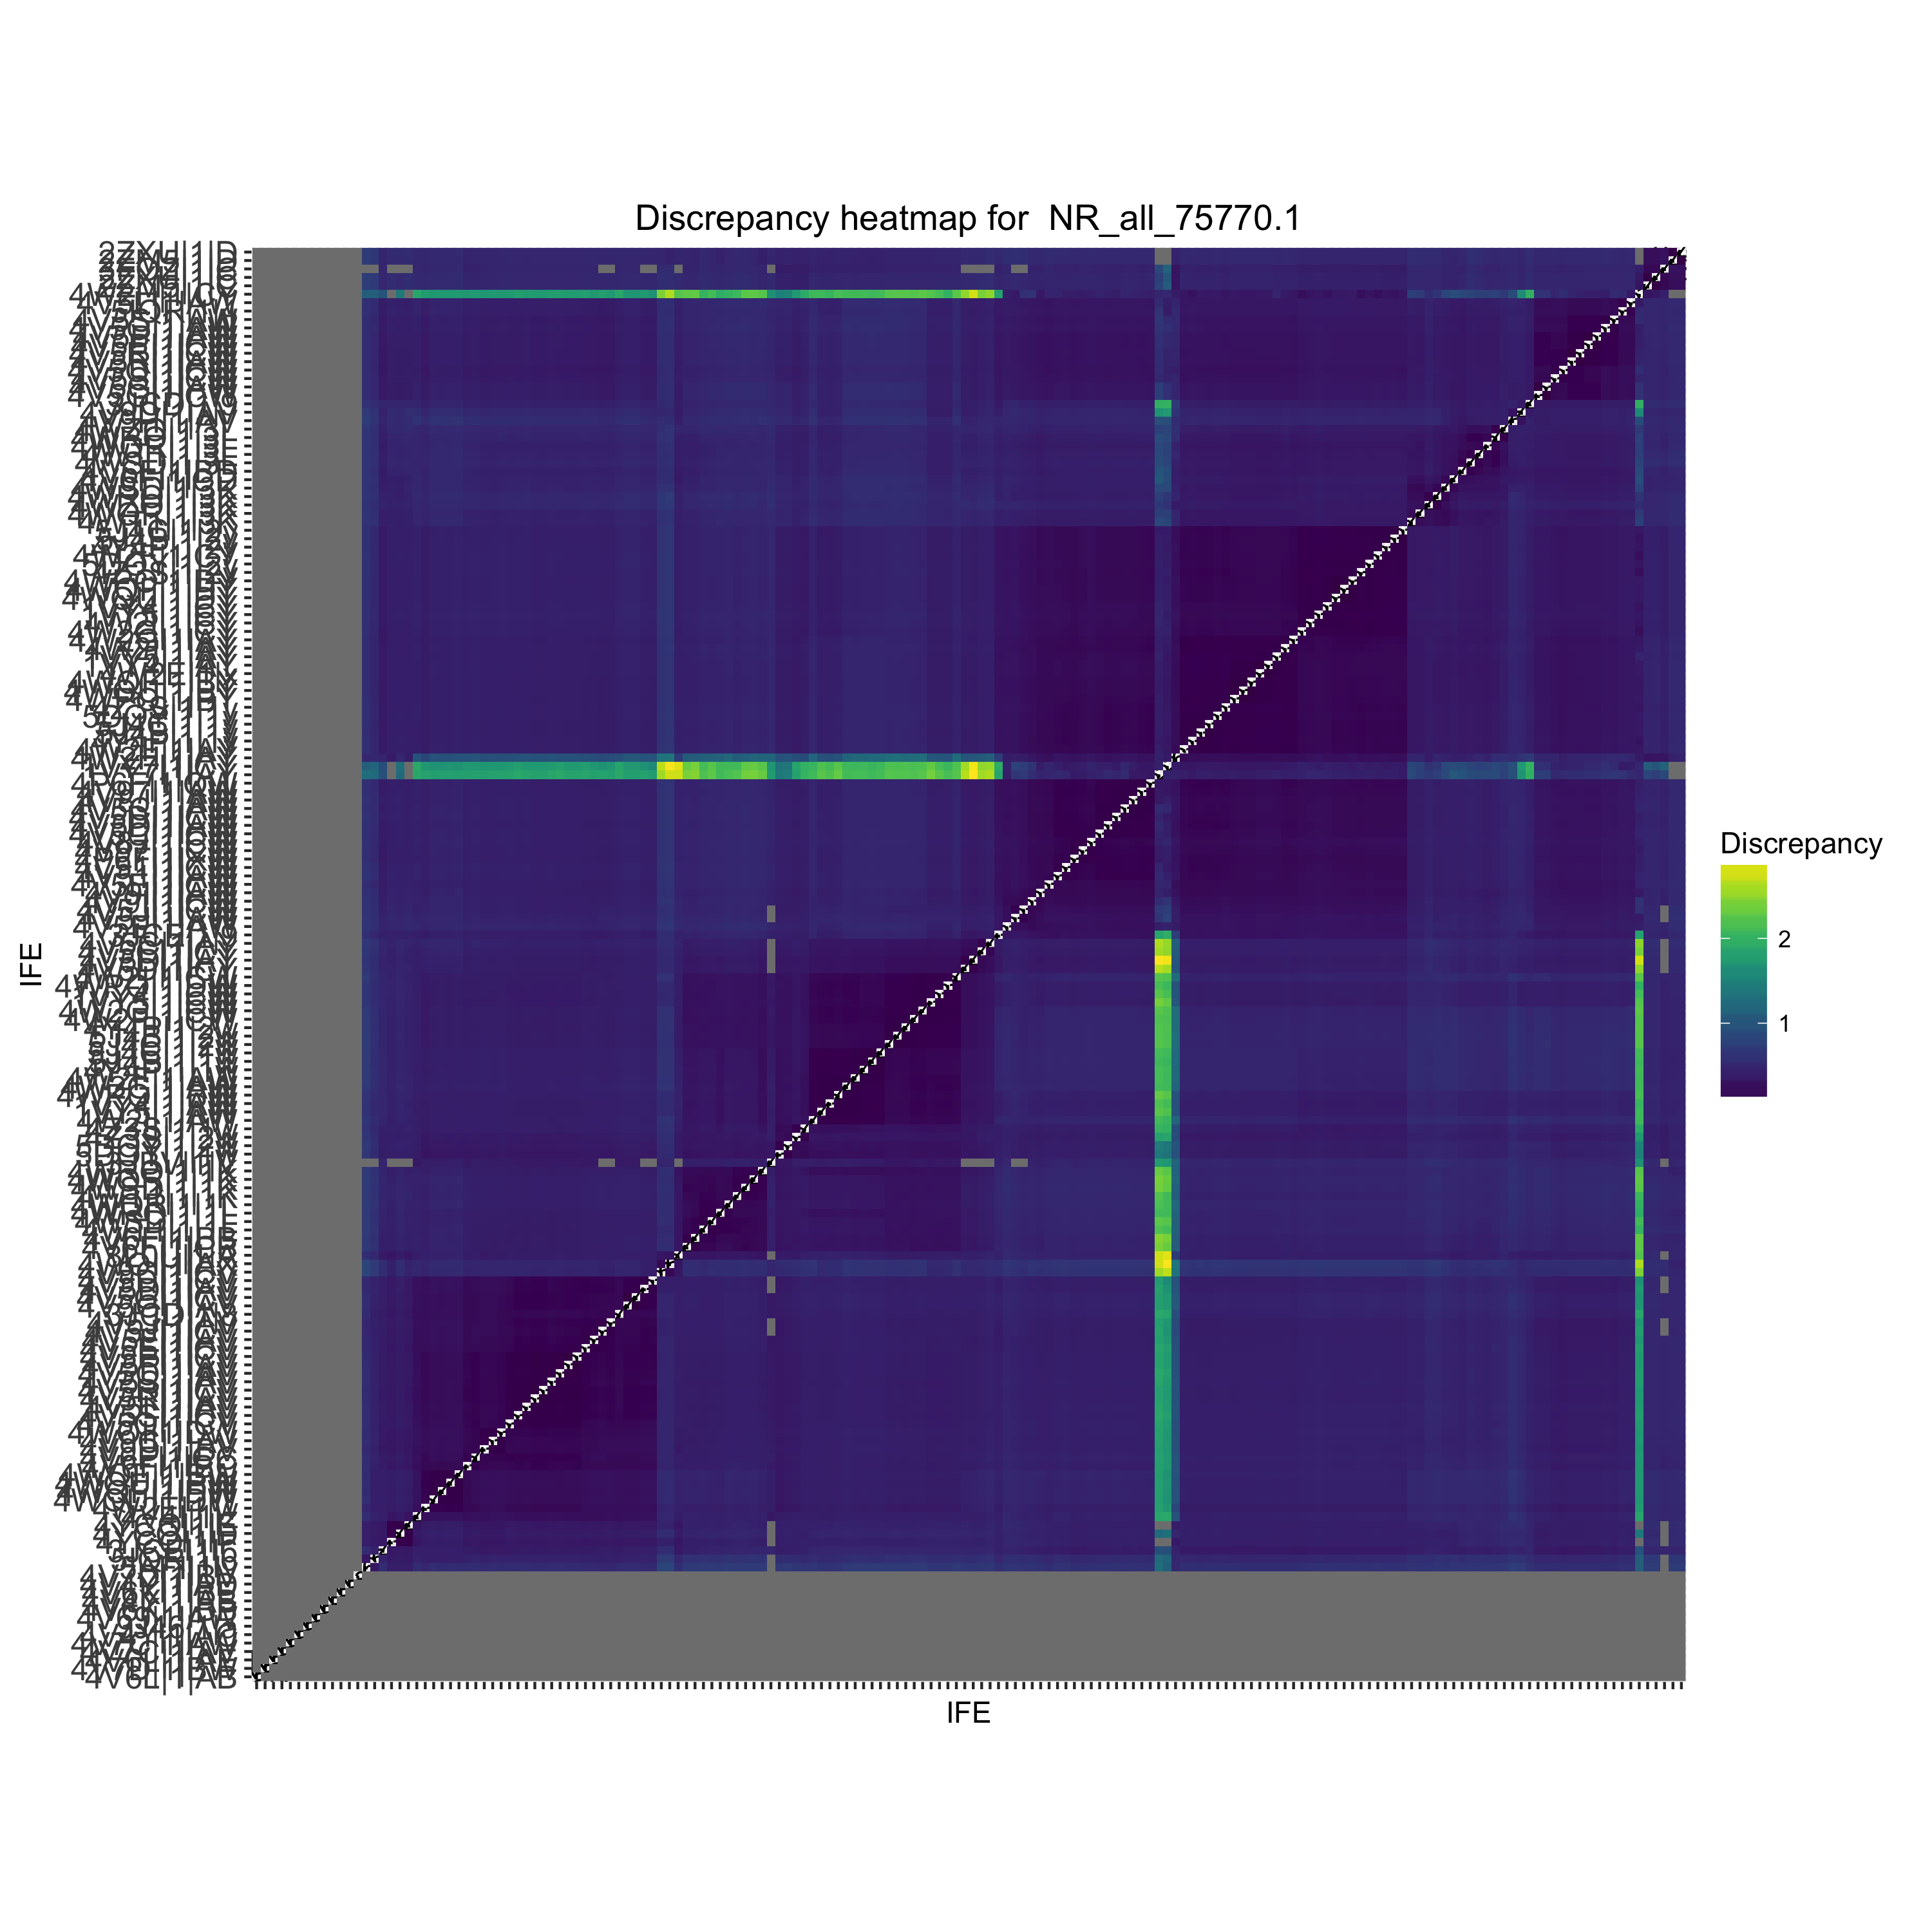
\includegraphics[width=\linewidth]{chapter-3/figs/nr-all-75770-1-disc}
  \caption{Histogram of the of the discrepancies for EC NR\_all\_75770.1, an E.
    coli tRNA group. This group contains a few IFE's which are outliers in our
  analysis.}
  \label{fig:nr-all-75770.1-disc}
\end{figure}

The other possibility is that the chains are connected through an IFE for which
geometric discrepancy was not computed. An example of this is show in
Figure~\ref{fig:nr-all-18070.1-disc}. In this figure we can see a yellow line in
the upper right which covers the entire heatmap. This indicates that this IFE
has high geometric discrepancy to all other members of the group. This IFE is connected to
all other members through the IFE's that have no geometric discrepancy shown (grey bars).

I examined the two EC's, NR\_all\_18070.1 and NR\_all\_75770.1 and found that
they are tRNA EC's. NR\_all\_18070.1 which is a tRNA group with 233 members and
is the dot with the highest number of members on the summary graphs shown in
Figure~\ref{fig:outlier-detail}. Shown in Figure~\ref{fig:nr-all-18070.1-disc}.
The outliers are due to a single IFE which is a truncated tRNA. While it is
somewhat structurally different for the part that exists from all other members
it is very similar in experimental sequence. It is connected to the rest of the
chains through IFE's which have no computed geometric discrepancy.

\begin{figure}[h]
        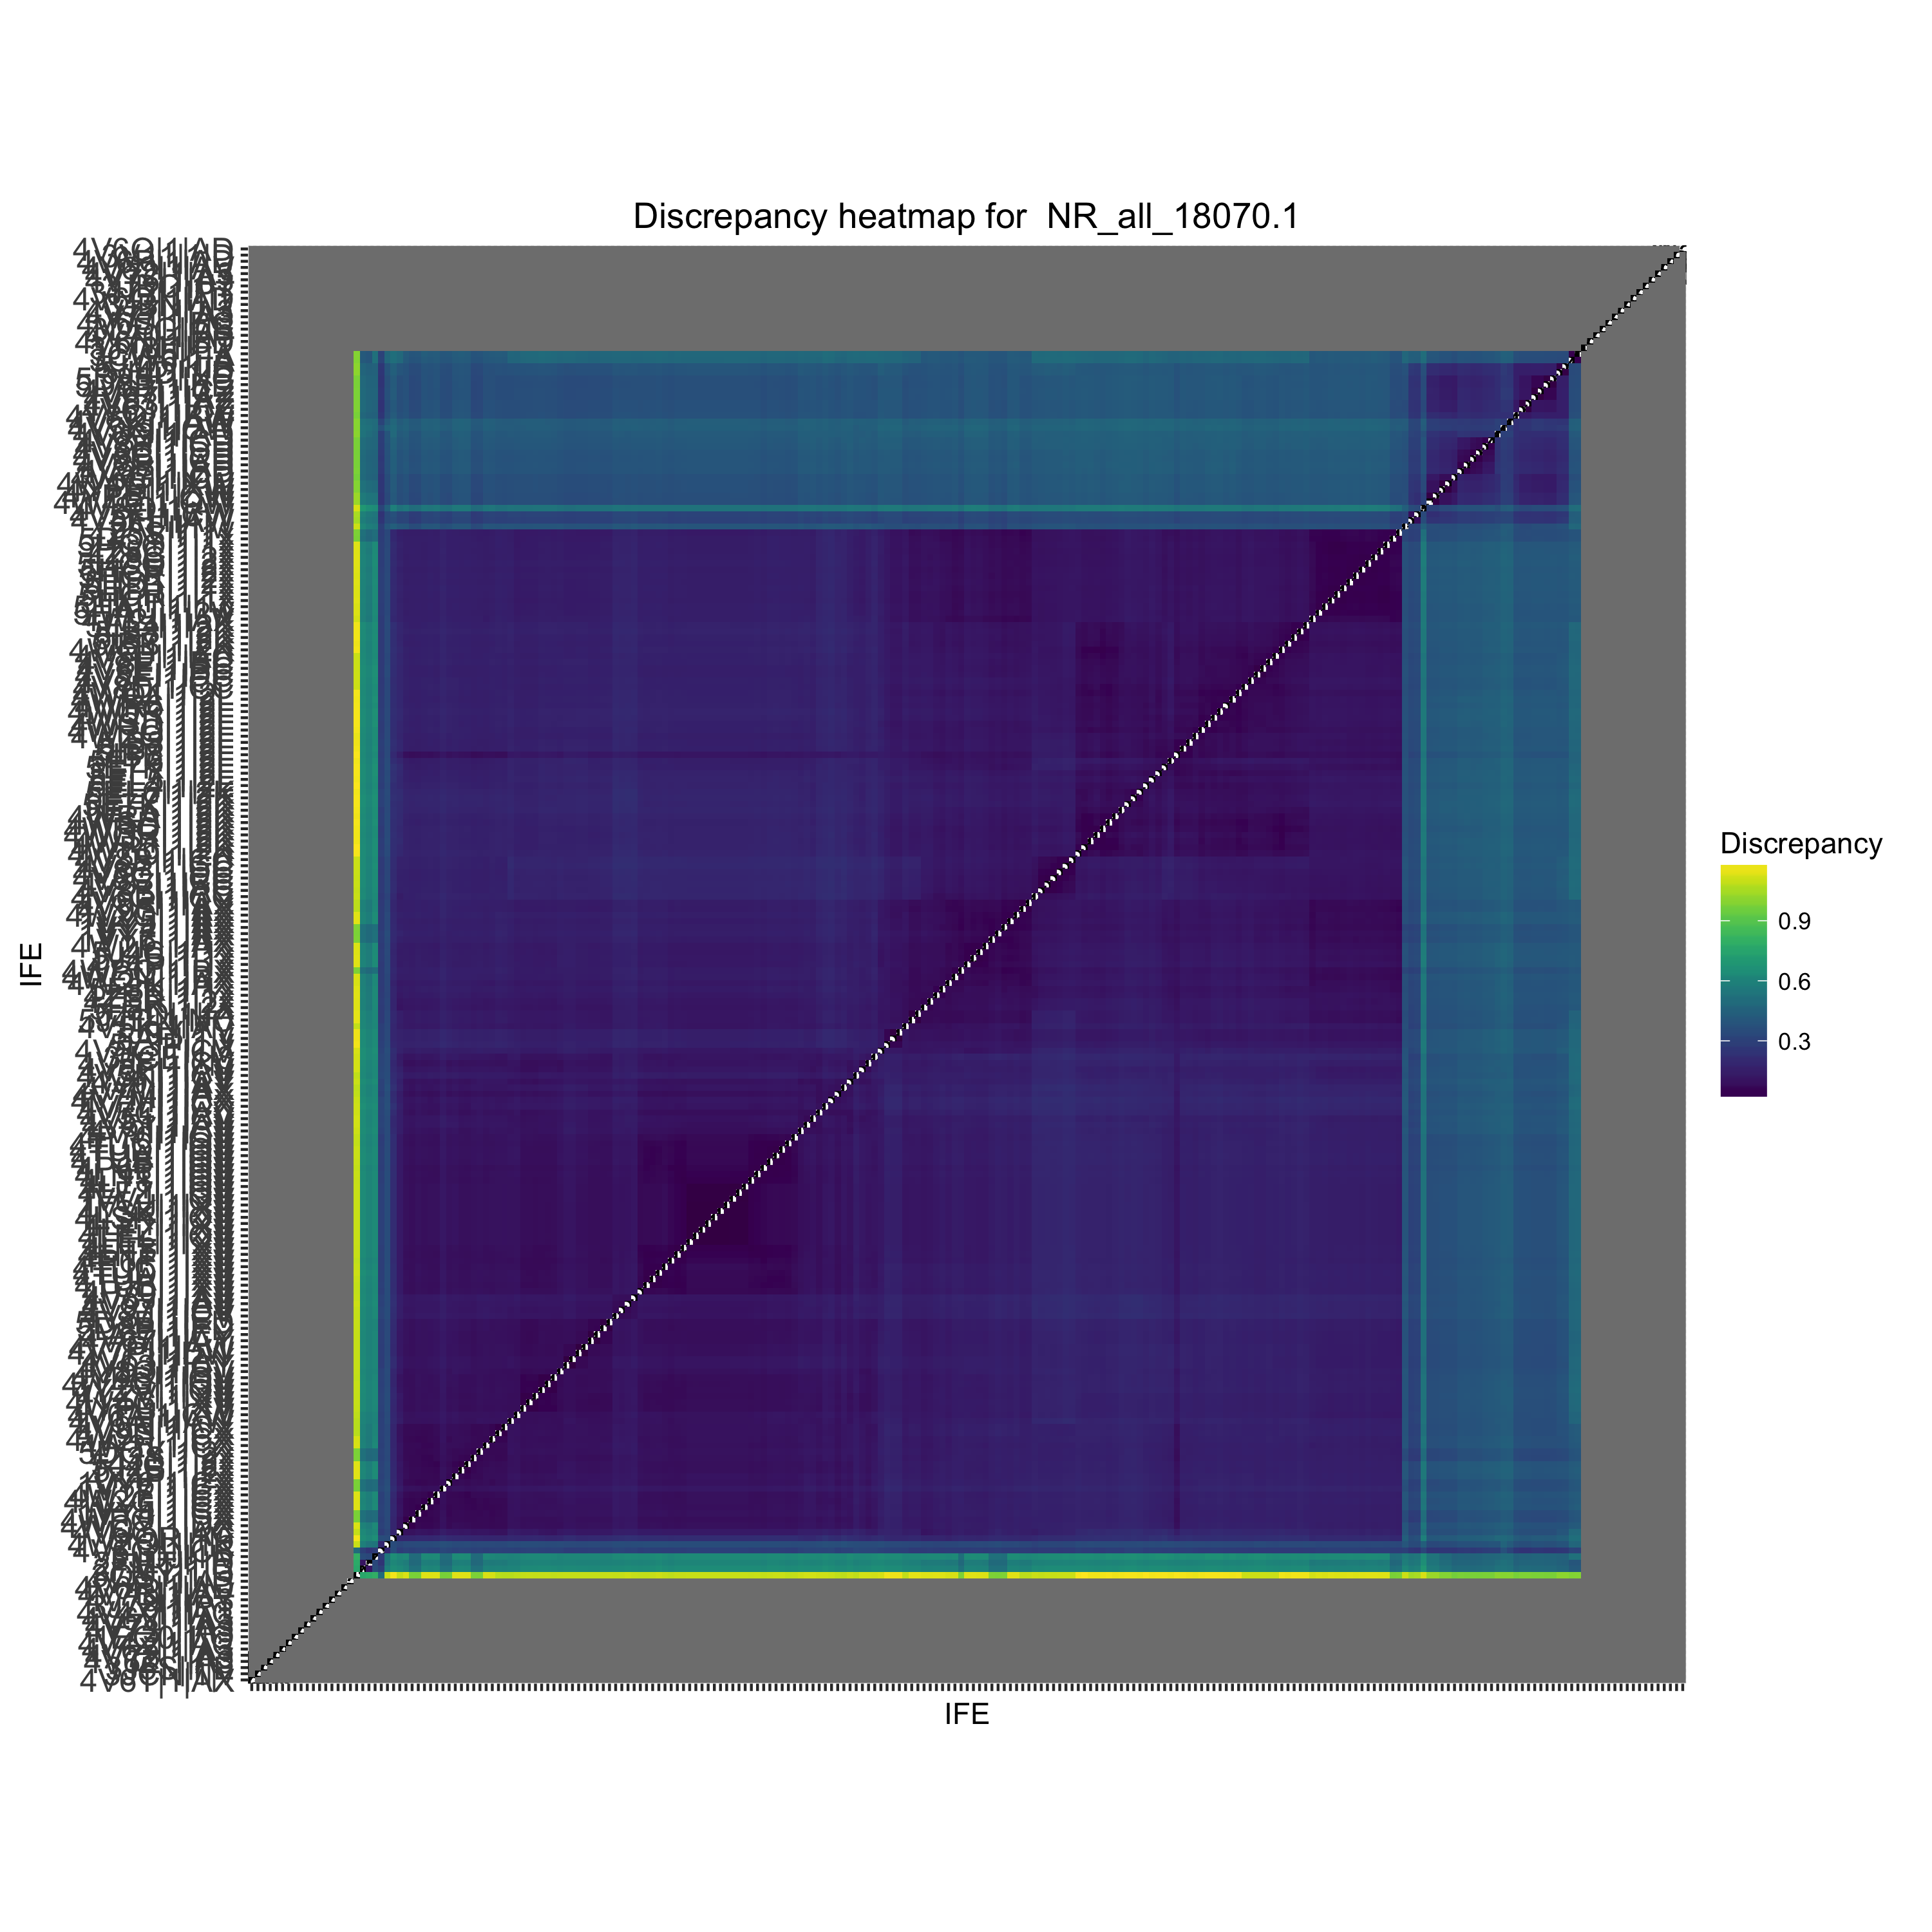
\includegraphics[width=\textwidth]{chapter-3/figs/nr-all-18070-1-disc}
  \caption{Figure summarizing the geometric discrepancy heatmap for all IFE's in
  NR\_all\_18070.1, a tRNA group with 233 members. }
  \label{fig:nr-all-18070.1-disc}
\end{figure}

NR\_all\_75770.1, the second highest point on Figure~\ref{fig:outlier-detail}.
It is an \EC{} tRNA group with 170 members. There are a few IFE's which are
outliers relative to the rest of the group, which appear to be fragments of the
larger tRNA. For example 1VY7 is a 5 nt fragment of the 76 nt tRNA. I do not
think 5 nt fragments of a tRNA are worth their own EC and thus believe such
fragments should be included with the complete IFE's as well.

I manually investigated the other EC with outliers and found that the outliers
are often placed into the same group because there is a structure for which
there is no computed geometric discrepancy for, such as a low resolution X-ray,
that connects the outliers to the rest of the group. For example, in previous
version where we did not compute geometric discrepancy for NMR structures, an
HIV hairpin would be joined with a duplex of the same sequence because there was
an NMR structure. All three types of chains, the duplex, hairpin and NMR
structure contained the same sequence and thus were joined on the basis of
sequence similarity. This was resolved for NMR structures with the adoption of
geometric discrepancy for them as well. However, it remains an issue for low
resolution X-ray crystallography experiments, but only for the lowest resolution
EC groups.

\section{Conclusions and future extensions}

Overall our grouping methodology for EC successfully groups all FE's into
coherent EC. Our methodology is an improvement over the previous approach for
several reasons. First, it can work take full advantage of mmCIF data by
extracting all chains, not just the longest RNA chain in a file. Secondly, it
computes discrepancies and alignments between all pairs of chains and stores
them in our database, to allow for future tuning of the parameters. Finally, our
method avoids unnecessary computation of discrepancies for low resolution
structures, which produce unusable data. 

There are several improvements that remain to be made. Notably, our method of
geometric similarity, geometric discrepancy, is flawed for this task. It is too
sensitive of poor modeling in structures. Often the issue is the orientations of
bases in nucleotides of low resolution structures. If this was replaced with a
different method that is less sensitive to base orientation it may be possible
to compute geometric comparisons between all pairs of IFE's, including those
determined at low resolution.

In addition, while evaluating the methodology it was very useful to compute EC's
using only sequences and then examine the changes when geometric discrepancy is
applied. This could become part of the standard clustering procedure. For
example it may be useful to create a series of groupings. First build the EC
only using sequence similarity,then add species constraints, then finally add
the geometric discrepancy comparisons. This would make it easier to examine our
methodology as well as provide information about the linkages, if any between
groups. For example, there are likely many small groups that differ structurally
but have the same, or very similar sequences. Such groups may be interesting for
researchers investigating the range of structures a single sequence can form. A
hierarchy of groupings could make this easier to determine.

Finally, small structures may well require a different set of rules for
comparison grouping. The work here was guided strongly by our experience with
rRNA's and tRNA molecules. These much larger RNA's show much clearer differences
than small synthetic molecules. It may be worthwhile to focus exclusively on the
small molecules to improve the methodology. For example, we currently only use
one chain when making geometric comparisons. This works well with large
molecules but may not be accurate for small synthetic compounds. In addition, it
may be better to allow small chains to join through non-canonical pairs as well
as canonical cWW pairs. Doing so could allow us to build better groups for the
poly-A duplex or G-quadruplexes more accurately.
